%!TEX option = --shell-escape

\documentclass[12pt,a4paper,oneside,final]{report} 		

% Nastavení formátu stránky a jazyková nastavení

\usepackage[utf8]{inputenc}		%čeština
\usepackage[czech]{babel}			%čeština
\usepackage[T1]{fontenc}			%čeština
\usepackage{nimbusserif}			%font
\usepackage[hidelinks]{hyperref}
\usepackage{lipsum}
\usepackage{tocloft}
\usepackage{csquotes}
% Možnost nastavení barvy odkazů
% \hypersetup{
%     colorlinks=true,
%     urlcolor=cyan,
%     linkcolor=green,
%     filecolor=red,
%     citecolor=red,
%     }

\usepackage[total={15cm,25cm}, top=2cm, left=3cm, includefoot]{geometry}	%okraje stránek
\setlength{\emergencystretch}{3em}
%\setlength{\headheight}{5pt}		
\clubpenalty 10000		%sirotci a vdovy
\widowpenalty 10000	%sirotci a vdovy
\setcounter{tocdepth}{2}                % počet úrovní v TOC
\setcounter{secnumdepth}{2}             % počet úrovní číslování kapitol

%-------------------------------------------------------------------------------------------------------------------------------
% Nastavení citací
\usepackage[citestyle=numeric, style=numeric]{biblatex}
\DeclareFieldFormat{labelnumber}{\textsuperscript{[#1]}}
\renewcommand*{\mkbibbrackets}[1]{#1}
\addbibresource{citace.bib}
%-------------------------------------------------------------------------------------------------------------------------------
% Nastavení tabulek a obrázků
\usepackage{adjustbox}	%možnosti šířky tabulky
\usepackage{graphicx,wrapfig,epsfig,subcaption}	%obrázky
\usepackage{amsmath,amsfonts,amssymb}	%matematika
\usepackage{enumitem}	%seznamy

\usepackage{multirow,array}	%tabulky
\newcolumntype{R}[1]{>{\raggedleft\let\newline\\\arraybackslash\hspace{0pt}}m{#1}}
\newcolumntype{P}[1]{>{\raggedright\arraybackslash}p{#1}}		%nastavení tabulek
\usepackage[font=small,labelfont=bf,textfont=it]{caption}	%Změna popisků
\renewcommand{\arraystretch}{1.5}							%Výška řádku
\usepackage[flushleft]{threeparttable}      % složitější tabulky
\usepackage{longtable}                      % dlouhé tabulky
\usepackage{bm}
\usepackage{booktabs}                       % knižní tabulky

% Nastavení cmidrule a cline pro babel
\usepackage{regexpatch}
\makeatletter
% Change the `-` delimiter to an active character
\xpatchparametertext\@@@cmidrule{-}{\cA-}{}{}
\xpatchparametertext\@cline{-}{\cA-}{}{}
\makeatother

\usepackage{lscape}                         % otočení objektu (obrázku, tabulky), včetně popisu
\usepackage{rotating}                       % rotace obektů
\usepackage{wrapfig}                        % umístění objektu do textu

\usepackage{siunitx}	%jednotky a jejich nastavení na češtinu
\sisetup{detect-all, output-decimal-marker = {,}, list-final-separator = { a~},inter-unit-product = \ensuremath{{}\cdot{}}, range-phrase=--}

%------------------------------------------------------------------------------------------------------------------------------
% Nastavení formátování stránky, záhlaví a zápatí
\usepackage{fancyhdr}	%záhlaví a zápatí
\usepackage{setspace}
\setstretch{1.5}
\newcommand{\helv}						%---Písmo
	{
		\fontshape{it}					%---Kurzíva			
		\fontsize{12}{12}				%---Velikost
		\selectfont
	}	

\usepackage{titlesec}

\titleformat{\chapter}{\bfseries\huge}{\thechapter}{16pt}{}
\titlespacing*{\chapter}{0pt}{0ex plus 0ex minus .2ex}{1.5ex plus .2ex}

\newcommand{\clear}{
    \fancypagestyle{plain}{%
        \fancyhf{}                          % clear all header and footer fields
        \rfoot{\helv \thepage}
    }
}

\fancypagestyle{plain}{
					\fancyhf{}								
					\fancyfoot[R]{\helv \thepage}			
					
				}

%předefinování záhlaví a zápatí
\fancyhf{}								%---Vymaže záhlaví/zápatí
\lhead{}								%---Levé záhlaví
\chead{}								%---Střed záhlaví
\rhead{\helv \nouppercase{\nazevCZ}}	%---Pravé záhlaví
\lfoot{}								%---Levé zápatí
\cfoot{}					            %---Střed zápatí (číslo stránky)
\rfoot{\helv \thepage}					%---Pravé zápatí
\setlength{\headheight}{15pt}

\pagestyle{fancy} \def\thepage{\arabic{page}}


%-------------------------------------------------------------------------------------------------------------------------------
% Nastavení psaní kódu
\usepackage{listings}
\usepackage{xcolor}

\definecolor{codegreen}{rgb}{0,0.6,0}
\definecolor{codegray}{rgb}{0.5,0.5,0.5}
\definecolor{codepurple}{rgb}{0.58,0,0.82}
\definecolor{backcolour}{rgb}{0.95,0.95,0.92}

\lstdefinestyle{mystyle}{
    backgroundcolor=\color{backcolour},   
    commentstyle=\color{codegreen},
    keywordstyle=\color{magenta},
    numberstyle=\tiny\color{codegray},
    stringstyle=\color{codepurple},
    basicstyle=\ttfamily\footnotesize,
    breakatwhitespace=false,         
    breaklines=true,                 
    captionpos=b,                    
    keepspaces=true,                 
    numbers=left,                    
    numbersep=5pt,                  
    showspaces=false,                
    showstringspaces=false,
    showtabs=false,                  
    tabsize=2
}

\lstset{style=mystyle}

\newenvironment{shortitemize}[1][\textbullet]{%
    \begin{itemize}[label={#1}]
        \setlength{\itemsep}{0pt}
        \setlength{\parskip}{0pt}
        \setlength{\parsep}{0pt}
}{%
    \end{itemize}
}
\usepackage{pdfpages} % titulní strana
\usepackage{todonotes}
    % Nastavení vzhledu. Soubory v adresáři data neměňte, pokud to není nutné!

%-----------------------------------------------------------------------------------------------------------------------------
%--- Zkratky – Vyplnit potřebné informace v závorkách!!!

\newcommand{\skola}{Vyšší odborná škola a Střední průmyslová \\škola elektrotechnická Olomouc,\\ Božetěchova 3}

\newcommand{\typPrace}{DLOUHODOBÁ MATURITNÍ PRÁCE}      
\newcommand{\nazevCZ}{Programování stránek pro Worldee.com}                      % Název práce v českém jazyce
\newcommand{\autor}{Jan Dlabaja}                        % Jméno autora
\newcommand{\vedouci}{Bc. Martin Meravý}         % Jméno vedoucího práce i s tituly
%-----------------------------------------------------------------------------------------------------------------------------
% Neměňte tuto část

\begin{document}
	\setlength{\headheight}{64pt}

\fancypagestyle{titulka}{
	\fancyhf{}								%---Vymaže záhlaví/zápatí
	\lhead{\includegraphics[width=3cm]{data/logo školy.png}}
	\renewcommand{\headrulewidth}{0pt}	%---Horní čára
	\renewcommand{\footrulewidth}{0pt}	%---Dolní čára
}
\pagestyle{titulka}

\begin{center}
	\vspace{1cm}
		\large{\textbf{\skola}}
	\par	
	\vspace{7cm} \par	
		\large{\textbf{\typPrace}}
	\par
		\parbox[t]{12cm}{\center\large{\nazevCZ}}
	\vspace{6cm} \par
\end{center}


\begin{tabular}{ll}
	Autor práce: & \textbf{\autor}	\\
        Obor: & \textbf{Technické lyceum}	\\
	Vedoucí práce: & \textbf{\vedouci} \\
	Školní rok: & \textbf{2024/2025} \\
\end{tabular}		

\vspace{1cm}
        \newpage
\setlength{\headheight}{0pt}
\thispagestyle{empty}

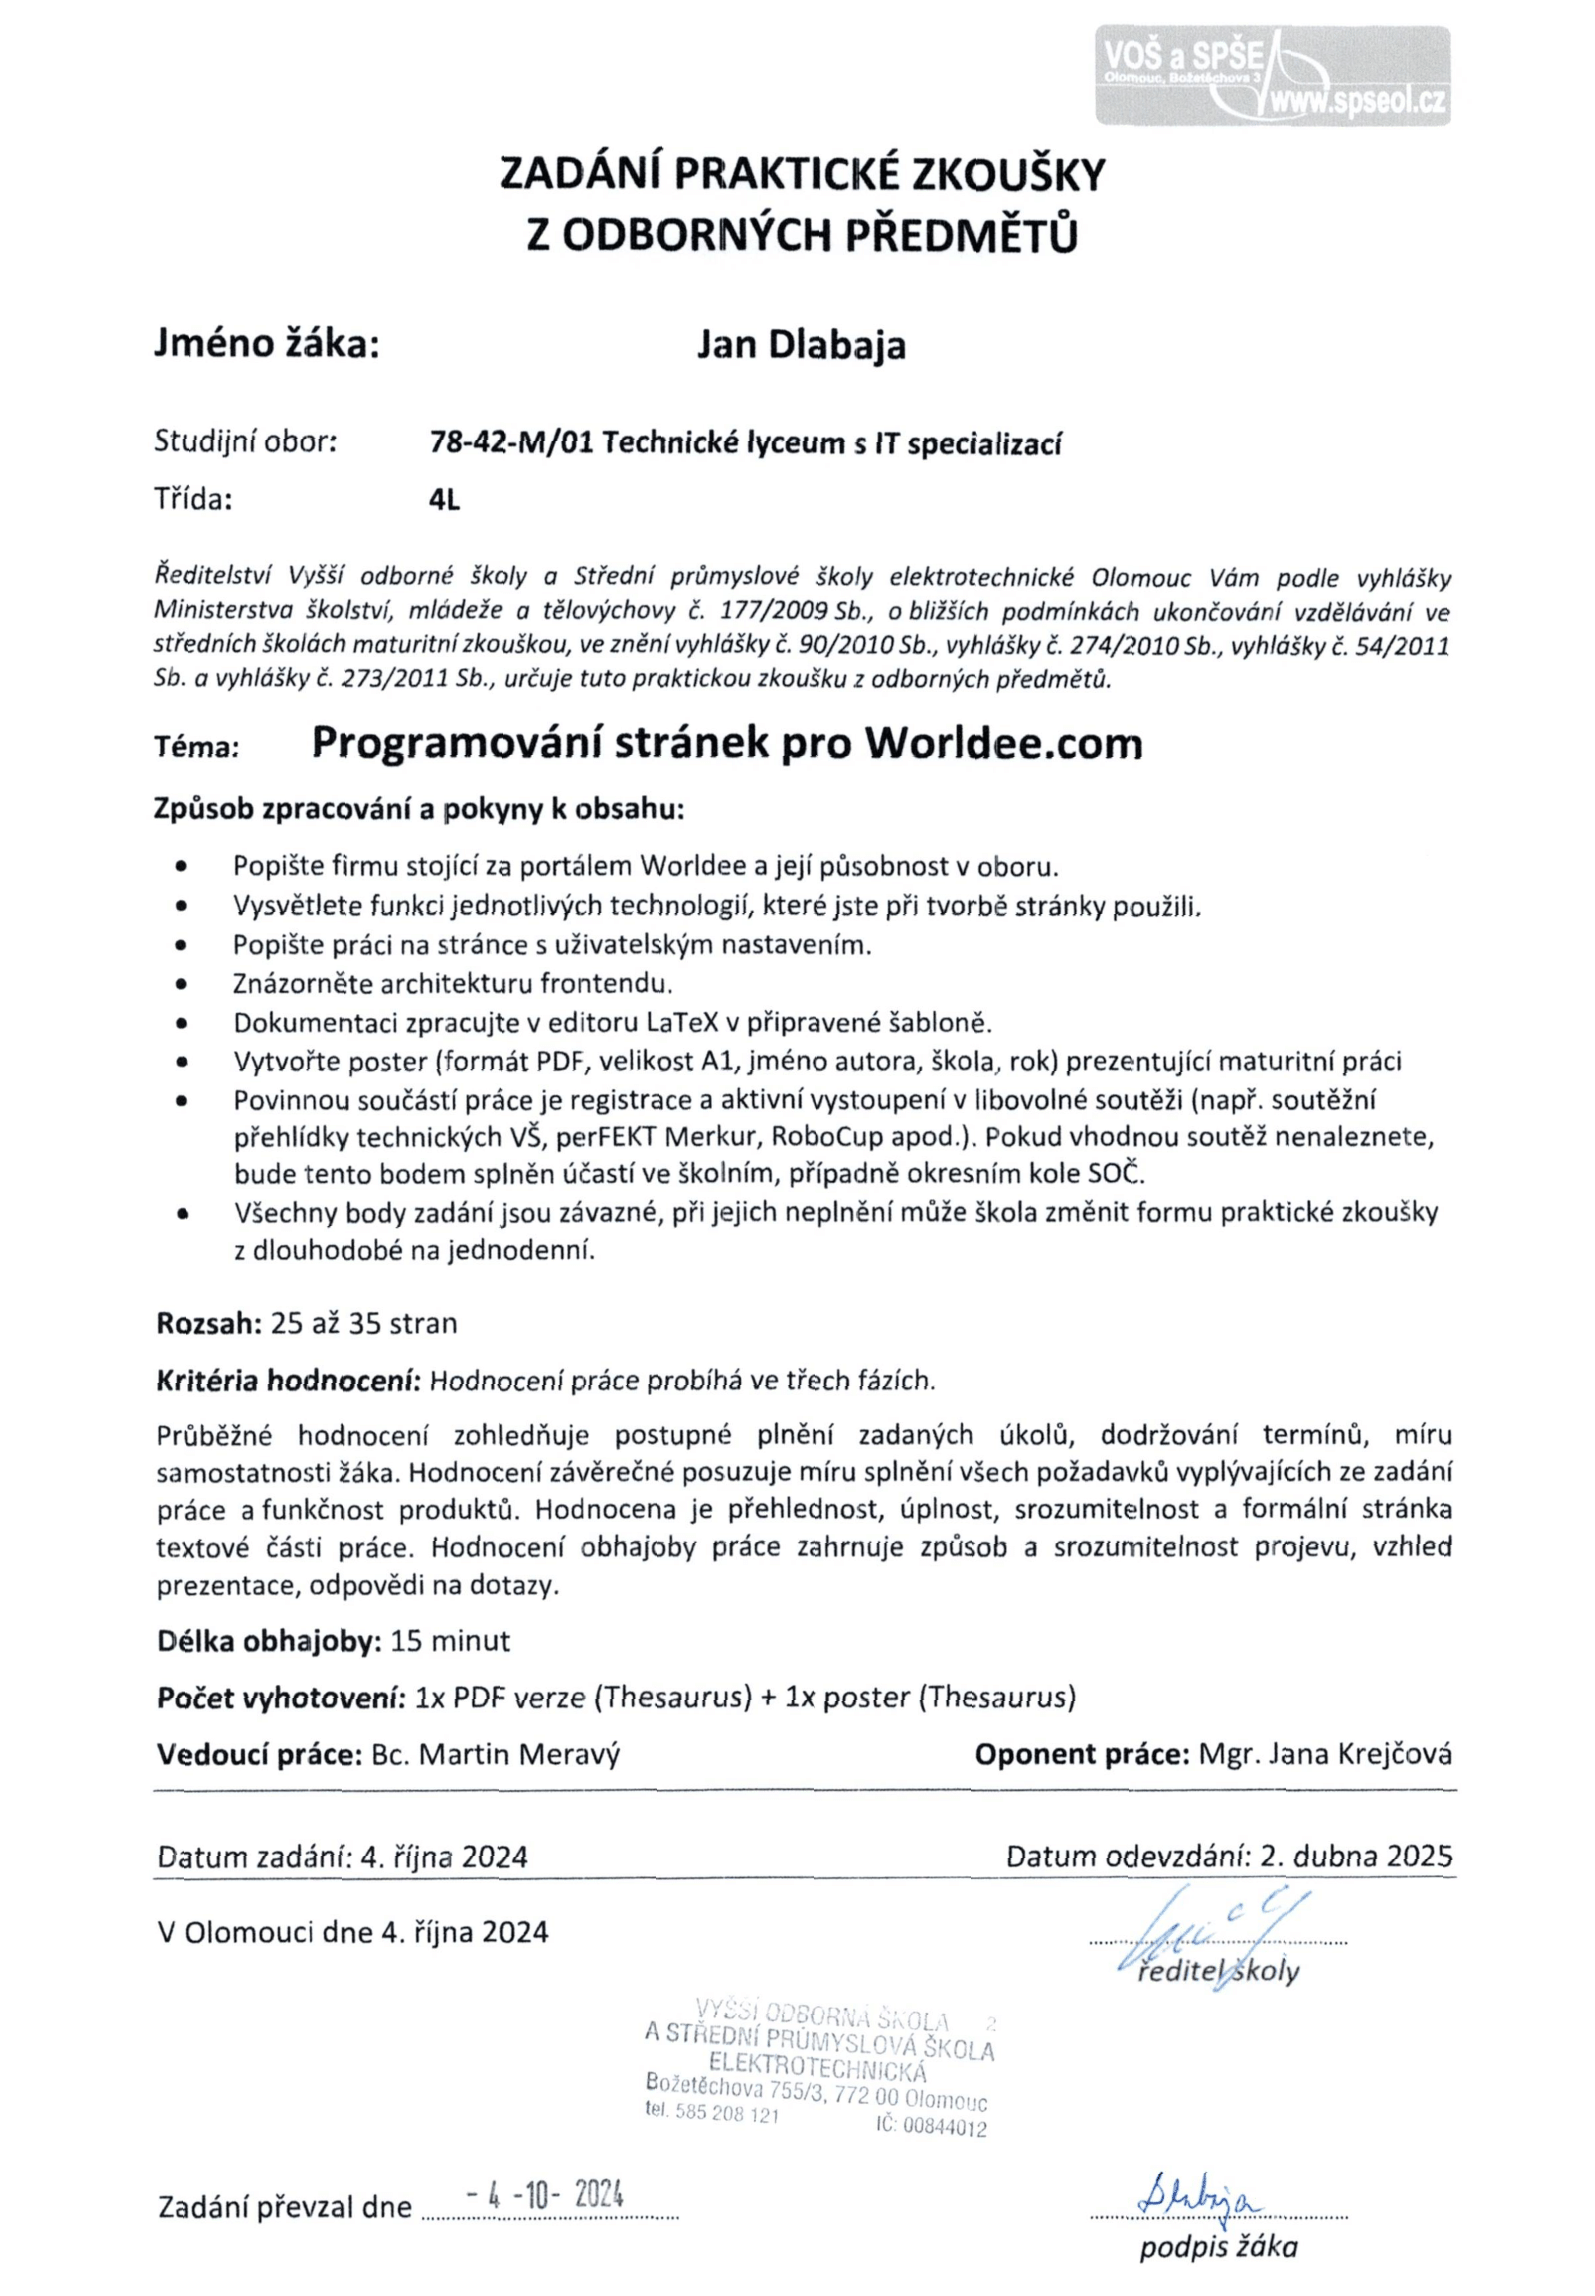
\includepdf{data/zadani.png}
	\newpage
\thispagestyle{empty}
\setlength{\headheight}{64pt}


\vspace{8cm} 			
\noindent Prohlašuji, že jsem seminární práci vypracoval samostatně a~všechny prameny jsem uvedl v~seznamu použité literatury.
\par
\vspace{5mm}\hfill
    \begin{tabular}{c}
    	\\                               
    	........................................\\       
    	\autor                                           
    \end{tabular}  
    \par

\vspace{2cm} 			
\noindent Prohlašuji, že nemám námitek proti půjčování nebo zveřejňování mé práce nebo její části se souhlasem školy.
\par
\vspace{5mm}\hfill
    \begin{tabular}{c}
    	\\                               
    	........................................\\       
    	\autor                                           
    \end{tabular}  
    \par

\vspace{2cm} 			
\noindent Chtěl bych vyslovit poděkování Bc. Martinu Meravému za odborné konzultace a poskytnuté informace. Také bych chtěl poděkovat panu Tomáši Zapletalovi za podklady k první kapitole.
\par
\vspace{5mm}\hfill
    \begin{tabular}{c}
    	\\                               
    	........................................\\       
    	\autor                                          
    \end{tabular}  
    \par
	
    %--- Obsah
    \tableofcontents
    \thispagestyle{empty}
    
    %------------------------------------------------------------------------------------------------------------------------------
    %--- Text dokumentu - každá položka odkazuje na jednu kapitolu nebo oddíl. Upravte názvy kapitol, uberte, přidejte podle potřeby.
    
    \chapter*{Úvod}\addcontentsline{toc}{chapter}{Úvod}\markboth{Úvod}{}

Asi spousta z vás už někdy vytvořila webovou stránku. Někteří z vás k její tvorbě dokonce využili i jeden z frameworků. Jak hluboko ale tato králičí nora jménem tvorba frontendu vlastně může jít?

Podobnou otázku jsem si pokládal koncem května 2024 po vstupu do startupu Worldee. Z webu jsem uměl jen HTML, CSS a základy JavaScriptu a zhruba tušil, k čemu je Sass. Během léta jsem si nejen tyto znalosti upevnil, ale navíc se naučil i pro mě úplně nové technologie, jako TypeScript, React, MobX, Next.js, nebo práci se Storybookem. Nakonec jsem v těchto technologiích vytvořil stránku s uživatelským nastavením, která bude na webu Worldee ještě několik dalších let. A přesně o tom bude tato práce.

V první kapitole se pokusím objasnit, co je prací a posláním společnosti. Pojem \uv{cestovka 2.0} nebo \uv{cestovatelská platforma} je totiž sice docela jednoznačný, ale zdaleka nepokrývá vše, co firma dělá. V další kapitole se pokusím popsat jednotlivé technologie, od těch základních, které většina lidí zná, jako HTML, CSS a JavaScript, přes
ty pokročilejší, jako React, TypeScript, nebo Next.js, až po některé nástroje používané na denní bázi, například next-intl a Jest. A nakonec se pokusím tvorbu takové stránky objasnit. S jakými komponentami jsem pracoval, jaké designy jsem skládal a jak vypadá jejich datová struktura. Řada přijde i na zmíněnou ukázku architektury webu.

Ale nyní – co je to to Worldee, jak vzniklo, a proč má potenciál stát se příštím \uv{jednorožcem}?
    \fancyhf{}
\rfoot{\helv \thepage}

\chapter{Firma Worldee}

\section{O firmě}

Co je vlastně to Worldee? Na to jsem si sám dlouho pokládal otázku. Jak jsem již říkal, ve zkratce je to taková cestovka 2.0. Nejlépe to ale asi popíše Tomáš Zapletal, její zakladatel, o nějž se v této části práce budu opírat.\cite{WorldeeInfo}

„Členové týmu Worldee vytváří platformu, která umožňuje lidem jednoduše objevovat svět. Spojením autenticity a jednoduchosti může díky naší platformě kdokoliv objevit téměř jakékoliv místo na zemi a cestovat v tom pravém slova smyslu. Naše poslání je ukázat lidem opravdový svět a pomoci jim odemknout skutečný potenciál jejich osobnosti - skrze zážitky, technologii a dokonalou zákaznickou zkušenost.“

A jak to vlastně funguje? Worldee je takový hybrid mezi sociální sítí a cestovní kanceláří, který se skvěle doplňuje. Itineráře na stránce tvoří sami uživatelé a zkušení cestovatelé, a pokud se Vám nějaký líbí, můžete si ho koupit. Worldee vyřídí vše od letenek, ubytování, auta a dalších služeb. Zároveň můžete cestovat s průvodcem nebo na vlastní pěst, s čímž Vám pomůže jejich mobilní aplikace.

Cíl je jediný – stejně jako si pod rezervací hotelů představí člověk Booking.com, tak pod itineráři by se Vám mělo vybavit právě Worldee.
\\
\begin{figure}[!h]
    \centering
    
\includegraphics[width=0.3\linewidth]{obrazky/worldee.png}
    \caption[Logo firmy Worldee]{Logo firmy Worldee\cite{Worldee}}
\end{figure}
\newpage
\section{Historie}

Vše začalo, když zakladatel firmy, Tomáš Zapletal, potřeboval někam nahrát své zážitky z cest.

\begin{displayquote}
Jiné sociální sítě k ukládání cestovatelských zážitků (celých itinerářů) nebyly uzpůsobené. Facebook, Instagram, ani jiná sociální síť. No a vzhledem k tomu, že jsem žádnou takovou, která by mi vyhovovala, nenašel, založil jsem ji sám.
\end{displayquote}

První prototyp vznikl v roce 2019 a vyvíjela ho externí firma, které Tomáš zaplatil asi dva miliony korun. Po prvním týdnu dostal na stránku přes 1500 uživatelů, které přilákal publikovaný článek na portálu \href{https://jaknaletenky.cz/cesky-startup-worldee-miri-do-sveta-a-potrebuje-vasi-pomoc.html}{jaknaletenky.cz}. K tomu vydal i \href{https://youtu.be/wJCV-5x0aIk}{první video} na \href{https://www.youtube.com/@worldee8910}{YouTube kanál Worldee}.

Časem bohužel zjistil, že se bez investice Worldee neposune. Společně se spoluzakladatelem Tomášem Nakládalem jezdili po republice a pokoušeli se získat 400 tisíc euro, které nakonec získali od Ondřeje Průši, zakladatele firmy prodávající známé Prusa 3D tiskárny.

První tým jedenácti lidí se v kanceláři poprvé sešel 1. 7. 2020. Vývoj a akvizice nových uživatelů šly pomalu. Největším problémem se ukázala být monetizace.

\begin{displayquote}
Už existovalo mnoho startupů, které měly podobně ušlechtilou myšlenku - pomáhat lidem objevovat svět, pomocí plánovače, nebo cestovatelského deníku. Všechny ale shořely ve chvíli, kdy chtěly nápad monetizovat. Budoucnost tedy byla jasná - nejtěžším úkolem pro nás bude postavit kolem tohoto nápadu udržitelný business.
\end{displayquote}

Nápad udělat z Worldee sociální síť tak částečně zkrachoval. Dobře nedopadl ani pokus o monetizaci mobilní aplikace. Jako nejlepší řešení se nakonec ukázalo prodej cest – pokud se Vám nějaký itinerář líbí, můžete si ho koupit jako balíček a bez starostí se na tu samou cestu vydat také. Byl to úspěch a první zájezd se vyprodal do 48\,hodin.

A tím se pomalu dostávám do současnosti, kdy jsem nastoupil i já. S Worldee byl ve Skotsku už i YouTuber Kovy se svým přítelem Mírou\cite{WorldeeKovy} a během toho přišla další, tentokrát stomilionová investice.\cite{WorldeeInvestice} Přispěl do ní zakladatel portálu Bazoš.cz Radim Smička a již podruhé společnost Kaiperi Venture Capital. Pomalu se rozjíždí expanze do zahraničí a tým se rozrostl na více než padesát lidí. A jak říká název jedné z Tomášem zaregistrovaných firem – \uv{The sky is no longer the limit (s.\,r.\,o.)}.\cite{Podnikani}

\newpage
\section{Produkty}

Pokud se s Worldee rozhodnete vydat na cestu, můžete si vybrat ze tří variant.\cite{Worldee}

\subsection*{Cesta s průvodcem}
    \begin{shortitemize}
        \item cesta s Čechem, který je se zákazníkem celou dobu od odletu po přílet
        \item v malé skupince (8 - 12 osob)
        \item v konkrétní termín
        \item musí se naplnit minimální kapacita cesty
    \end{shortitemize}
\subsection*{Cesta za expatem}
    \begin{shortitemize}
        \item cesta za Čechem, který se z ČR přestěhoval do zahraničí, kde si postavil/koupil malý rodinný hotel
        \item individuálně - je možné jet i v jedné osobě
        \item libovolný termín
        \item expat se o zákazníka celou dobu stará - vyzvedne ho na letišti, vaří mu, seznamuje ho s místními, radí mu, jaká místa navštívit. Stará se o to, aby destinaci opravdu autenticky poznal
    \end{shortitemize}
\subsection*{Self-guided itinerář}
    \begin{shortitemize}
        \item jakýkoliv itinerář lze zakoupit také jako self-guided itinerář a na cestu se vydat na vlastní pěst
        \item zákazníka neprovádí fyzická osoba, ale zkušený cestovatel zprostředkovaně přes aplikaci, do které už předem vše napsal
        \item na itinerář je možné jet kdykoliv, odkudkoliv na světě
    \end{shortitemize}
\newpage
\section{Business model a škálovatelnost}

Ještě pár let zpátky většinu modelu tvořilo premium, kterým si uživatel mohl vylepšit účet a získat několik výhod včetně většího místa na disku pro své cesty. To se ale ukázalo jako nedostatečné, a tak je dnes příjem tvořen prodejem itinerářů, za které si Worldee bere 25\% marži.

Aby mohly cesty s průvodcem vůbec fungovat, jsou všichni průvodci placení (např. 2000\,Kč na den) a vedení jako Travel Buddy. Těmi se může stát kdokoliv, kdo vyplní přihlašovací formulář a projde náborovým procesem. Podobné je to s expaty, jejichž odměna je již přímo zahrnuta v ceně služeb. Protože má Worldee licenci a pojištění proti úpadku, mohou portál průvodci použít pro legalizaci svého podnikání a zároveň si stále budovat svoji značku. Ačkoliv bude jejich škálovatelnost pro expanzi do zahraničí náročná, protože budou potřeba stovky lidí různých národností, žádná platforma, která by něco podobného nabízela, na globální úrovni zatím neexistuje. A přitom mají tito průvodci vysokou přidanou hodnotu, protože pomáhají zákazníkům překonat jazykovou bariéru a tím otevírají Worldee novým cílovým skupinám.

Daleko lépe škálovatelnější jsou cesty na vlastní pěst. Sám Tomáš o nich dokonce mluví jako o \uv{svatém grálu}. Vše by mělo do budoucna fungovat automaticky a data o hotelech, letenkách a autech brát od třetích stran. Všechny itineráře už Worldee nyní umí automaticky překládat do všech světových jazyků. Stačí, aby si zákazník vybral termín, a pak se nechal provádět mobilní aplikací v kapse.

\newpage
\section{Konkurence}

Ačkoliv je Worldee v Česku poměrně unikát, v zahraničí už existuje několik firem, které jsou s podobným projektem částečně úspěšné.

\subsection*{TripLegend} 
Jedná se o lokální německou cestovní kancelář založenou před čtyřmi lety. Nabízí cesty s průvodcem a spolupracují s cestovními agenturami, nedávno se začali pokoušet i o self-guided cesty. Zatím fungují v režimu break-even s jednotkami cest měsíčně, navíc bez jakéhokoliv vývojového týmu. Nicméně jsou důkazem, že podobný produkt může levně fungovat i na vysoce konkurenčním trhu.

\subsection*{\href{https://www.weroad.com/}{WeRoad}}
Tato cestovka má už mnohem větší dosah než TripLegend. Ačkoliv dělají jen cesty s~průvodcem doma a na některých západních trzích, a v balíčku ani nenabízí letenky, mají miliardový obrat a dokázali, že produkt může uspět i na chudším trhu, jako je Itálie.

\subsection*{\href{https://www.flashpack.com/}{FlashPack}}
Tento britský projekt, který se po pandemii dostal díky investorovi z insolvence, funguje hlavně na anglicky mluvících trzích. Staví si na prémiových službách a cenách, ale je možné, že se části z nich po saturaci trhu vzdají a díky penězům z marží expandují i na levnější trhy. Nicméně nemají ani vývojový tým, ani self-guided itineráře.

\subsection*{\href{https://www.polarsteps.com/}{PolarSteps}}
Jako poslední z firem tu uvedu projekt z Nizozemska. Podobně jako Worldee nabízí cestovatelský deník, ze kterého si ale navíc můžete nechat udělat fotoknihu. Zatím to pro Worldee může znamenat jen inspiraci pro další monetizaci, ale pokud své itineráře začnou prodávat, mohla by to být vzhledem k jejich velikosti potencionální hrozba.
\newpage
    \fancyhf{}
\rfoot{\helv \thepage}

\chapter{Použité webové technologie}
Než se dostanu k tvorbě samotné stránky, je potřeba si rozebrat technologie, které jsem k její tvorbě potřeboval a které mi značně ulehčily život. Půjdu postupně od nejjednodušších konceptů až k těm náročnějším a méně známým.

\section{HTML}

Na webu neexistuje důležitější technologie, než právě HTML. Bez tohoto značkovacího jazyku by na našem webu chyběl jakýkoliv obsah, slouží totiž k definování struktury stránky. Jeho syntax se skládá z párových (\texttt{<span>}potomek\texttt{</span>}) a nepárových (\texttt{<img/>}) značek, které se liší podle toho, zda v sobě obsahují potomky.

Zde je seznam několika základních elementů:

\begin{table}[h!]
\centering
\begin{tabular}{|>{\centering\arraybackslash}m{4cm}|>{\centering\arraybackslash}m{5cm}|}
\hline
\textbf{Element} & \textbf{Popis} \\ \hline
\texttt{span} & Jednoduchý text \\ \hline
\texttt{div} & Prázdný element \\ \hline
\texttt{p} & Odstavec \\ \hline
\texttt{button} & Tlačítko \\ \hline
\texttt{img} & Obrázek \\ \hline
\texttt{br} & Nový řádek \\ \hline
\texttt{h1, h2, h3, h4} & Nadpisy \\ \hline
\texttt{ol, ul} & Číslovaný/nečíslovaný seznam \\ \hline
\texttt{a} & Odkaz \\ \hline
\texttt{table} & Tabulka \\ \hline
\end{tabular}
\caption{Seznam základních elementů v HTML.}
\end{table}

Každý validní HTML dokument by měl mít dvě části. První je hlavička (head), ve které jsou definované informace, které na stránce nejsou vidět, jako její název, lokace skriptů a stylů, jazyk, font, nebo metadata. Druhá část je tělo (body). Tady už můžete používat všechny dříve zmíněné elementy a zobrazovat obsah samotné stránky.

Každý element má několik atributů, které můžete nastavit. \textit{Id} slouží jako unikátní identifikátor a \textit{class} zase reprezentuje skupinu prvků. Pomocí \textit{href} můžete prvku nastavit url adresu, a eventy jako \textit{onclick} nebo \textit{onmouseover} zase po splnění podmínky (kliknutí na element, přejetí myší) spustí definovaný skript.

V raných verzích se HTML dalo použít nejen k definování struktury stránky, ale i k jejímu stylování a pozicování jednotlivých elementů. Postupem času se ale toto paradigma stalo zbytečně komplexním, a tak se struktura a prezentace oddělily a vzniklo CSS.
\newpage
\section{CSS}

Styly vám na stránce umožní upravit téměř vše – měnit barvy, odsazení, pozice,
\mbox{velikost},~\ldots. Dají se psát buď do samostatných souborů s příponou \textit{.css}, do \texttt{<style></style>} elementu, nebo do \textit{style} atributu. Pro výběr konkrétních elementů se požívají tzv. selektory. Zde uvedu příklad na tlačítku.

\begin{table}[h!]
\centering
\begin{tabular}{|>{\ttfamily}m{4cm}|m{8cm}|}
\hline
\textbf{Selektor} & \textbf{Popis} \\ \hline
\texttt{button \{\}} & Změní všechny \texttt{<button/>} elementy na stránce \\ \hline
\texttt{.blue-button \{\}} & Změní všechny elementy se třídou (\textit{class}) \texttt{save-button} \\ \hline
\texttt{\#top-button \{\}} & Změní jeden konkrétní element s identifikátorem (\textit{id}) \texttt{top-button} \\ \hline
\end{tabular}
\caption{Příklady CSS selektorů a jejich funkcí.}
\end{table}

Do složených závorek následně můžete psát konkrétní styly. Například \texttt{background:~red;} nastaví pozadí prvku na červeno, \texttt{margin-right:~10px;} ho zase odsadí zprava o 10~pixelů, apod. Pokud chcete na element odkázat nepřímo, můžete za selektorem použít symboly \textit{>} (zaměřuje potomka) nebo \textit{<} (zaměřuje rodiče). Můžete také přídávat pseudo třídy jako \texttt{:hover} (změní element, pokud na něj najede kurzor myši), \texttt{:first-child} (aplikuje se na prvního potomka rodiče) a mnohé další. Pro potřeby pokročilých stylů se staly rozšířenými i pseudo elementy (\texttt{::before}, \texttt{::first-line}, \ldots). Jejich prací je vybrat konkrétní část elementu, například jeho potomka nebo první řádek.

Důležitou znalostí je také chápat box model a jeho jednotlivé části, které obklopují každý element. Jsou tři – vnitřní okraj (padding) určuje místo mezi obsahem a okrajem elementu (border), a vnější okraj (margin) zase oblast mezi elementem a ostatními prvky. U všech se dá nastavit velikost shora, zdola, zprava a zleva.

Pro responzivní design stránek, které se přizpůsobí jakékoliv obrazovce, vznikl počátkem minulého desetiletí flexbox. Ten konečně zjednodušil pozicování položek, které umožnil dávat do řádků nebo sloupců, zarovnávat je na začátek, střed, nebo konec, nastavovat mezi nimi mezery nebo je roztahovat pro zaplnění kontejneru.\cite{CSSFlexbox} Touto dobou také začala masová podpora media queries, které umožňují dynamicky měnit styly na základě aktuální velikosti stránky nebo vlastností displeje.
\newpage
\section{JavaScript}

Nástup JavaScriptu umožnil webovým vývojářům udržovat na stránkách aktuální data a~přidat interaktivní prvky, zlepšující uživatelský zážitek. 

Ačkoliv se to tak nemusí podle názvu zdát, JavaScript má s Javou jen pramálo společného. Vytvořil ho v roce 1995 během deseti dnů zaměstnanec firmy Netscape, tehdy ještě pod jménem Mocha a LiveScript. Java se do jména dostala až kvůli popularitě stejnojmenného jazyka. Standardy pro něj vyvíjí organizace Ecma International, podle níž se značí i jeho verze (ES5, ES6, \ldots).\cite{JSIntroduction}\cite{JSOrigins}\cite{JSHistory}

Protože se jedná o jediný jazyk, který umí prohlížeče číst, a zároveň je jednoduchý na pochopení i programování, docela rychle se rozšířil. O to více, když v roce 2009 vzniklo Node.js a umožnilo ho používat i mimo webové prostředí. Od té doby v něm lze napsat opravdu téměř vše a i díky velkému množství dostupných knihoven (například v online repozitáři \href{https://www.npmjs.com/}{NPM}) se těší vysoké popularitě.

JavaScript má dva typy proměnných – let (dá se měnit) a const (neměnná). Do nich lze přiřazovat různé zabudované typy jako boolean, number (64bitové desetinné číslo), bigInt, string, array, date, objekt a několik dalších. Existuje i tři prázdné typy, jako je \texttt{undefined} (bez přiřazené hodnoty), \texttt{null} (prázdá hodnota) a \texttt{NaN} (Not-a-Number, doslova \textit{není číslo}). Typy se nicméně kontrolují až při běhu, takže se na špatné přiřazení často přichází, až když je příliš pozdě.\cite{JSBasics}\cite{JSTypes}

Pokud píšete podmínky, musíte dávat pozor na porovnávání. Dvě rovnítka porovnávají typy, tři zase hodnoty. Záměnou prvního rovnítka za vykřičník vznikne negace. $\&\&$ značí logický operátor AND a $||$ zase OR. Některé typy (undefined, null, NaN, nebo prázdné řetězce) se označují jako \textit{falsy} a v podmínkách reprezentují hodnotu \texttt{false}. Dále můžete používat ternary operátory ($x\ ?\ y : z$, pokud je $x$ pravda, vykoná se $y$, jinak $z$) nebo jeho zkrácenou verzi ($x\ \&\&\ y$, pokud je $x$ falsy, vykoná se $y$), která se převážně používá v~Reactu pro podmíněné renderování.

Existuje i několik druhů cyklů. V obyčejném for cyklu nastavujete počáteční hodnotu, krok a podmínku, přičemž všechny argumenty jsou nepovinné. Nechybí ani podmíněný while a pro iteraci elementů v seznamu se nejlépe hodí forEach().

Jazyk umožňuje funkcionální i objektové programování. Třídy stejně jako u ostatních jazyků podporují konstruktory, dědičnost, zapouzdření, nebo interní metody (prefix \texttt{\#}). Objekty lze volně kombinovat s funkcemi. Ty mohou požadovat argumenty, které jsou buď kopií původních hodnot (primitivní typy), nebo referencí na původní proměnnou (objekty, pole, funkce). Každá funkce má návratový typ, který je v základu \texttt{undefined}.\cite{JSFunctions}\cite{JSFunctionalProgramming}
\newpage
\section{TypeScript}

TypeScript vznikl jako reakce na některé problémy s vývojem v JavaScriptu, primárně dynamickou kontrolu typů. Používá se pouze během vývoje a při bundlingu se transpiluje do JavaScriptu, aby ho prohlížeče dokázaly číst a spustit.

Již zmiňovanou výhodou a hlavním prodejním bodem je typová podpora. Výhodou dynamicky typovaného jazyka sice může být vyšší rychlost vývoje, ta ale (společně s~programem) padá, jakmile se nesprávný typ dostane do produkčního prostředí. Pokud to tak není podle použití zřejmé, musíte typ přímo definovat nebo použít \texttt{any}, které bude TypeScript ignorovat. Po spuštění pak staticky analyzuje celý kód a pokud najde chybu, odmítne ho sestavit.

S typy lze dělat mnoho operací. Spousta z nich je postavená na obecných typech, umožňujících bezpečně použít více než jeden typ.\cite{TSGenerics}. Například \texttt{Omit<Typ, Parametry>} umožňuje z typu odstranit určité parametry a pomocí \texttt{Pick} je zase přidat. \texttt{Partial<Typ>} zase narozdíl od \texttt{Required} všechny parametry udělá nepovinné, \texttt{Readonly} je nastaví jen pro čtení a \texttt{NonNullable} odstraní všechny hodnoty s \texttt{null} nebo \texttt{undefined} typem. S~typy lze dělat i logické operace, jako průnik nebo sjednocení.

S udržováním všech typů vám mohou pomoci interfacy, ve kterých můžete například definovat parametry pro funkce a metody a následně je (jako šablony) znovupoužít na dalších místech v projektu.

TypeScript přidává i rozšířenou podporu enumů, které umožňuje definovat sadu pojmenovaných konstant. Hodnota každé položky může být \texttt{number} nebo \texttt{string}.\cite{WhatIsAnEnum}

V neposlední řadě jazyk přidává nové funkce pro třídy. Nad metodami nyní můžete volat dekorátory modifikující jejich chování, nebo vytvořit nové se stejným jménem ale jinými argumenty a metodu takzvaně \enquote{přetížit}. Zatímco dekorátory mají prefix @, u~interních funkcí nutnost prefixu odpadá a nahrazuje ho klíčové slovo \texttt{private}. Pro ještě lepší zážitek z OOP lze používat abstraktní třídy, které nelze instancovat, ale jejichž implementaci mohou využít všichni její potomci.
\newpage
\section{Sass, Less a moduly}

O CSS už jste četli. A i tato technologie má překvapivě pár nevýhod. Jedna z největších je fakt, že nemůžete znovu použít už napsaný kód. Takže pokud chcete na více místech tučné bílé písmo o velikosti 12 pixelů, musíte ho vždy znovu definovat. A pokud si po nějakém čase uvědomíte, že by písmo mělo být větší, nezbývá Vám nic jiného, než jeho výšku na všech místech změnit a doufat, že jste na nic nezapomněl.

Tohle už se zřejmě několika lidem stalo, proto v roce 2006 vzniknul Sass\cite{Sass} a brzy po něm Less\cite{Less}. Podobně jako TypeScript se jednalo pouze o nadstavbu nad stávající jazyk, který se v tomto případě zkompiloval do CSS. Dokázal ale vyřešit několik do té doby neřešitelných problémů.

Proměnné usnadnily život nejednomu programátorovi. Pokud si designér na poslední chvíli rozmyslel velikost fontu, stačilo ho změnit jen na jednom místě. K tomu se vážou i mixiny – malé části kódu, na které se dá kdekoliv odkázat. Navíc přijímají i parametry, umožňující přizpůsobit chování mixinu zvenku. Kromě toho tyto nadstavby zvládají aplikovat jednotlivé styly v závislosti na podmínkách, umožňují používat cykly (většinou pro aplikování stylů na třídy a identifikátory s podobným názvem), a také dokáží zpracovat vnořování jednotlivých stylů, což dělá soubory menší a kód čitelnější.

Jako poslední zmíním CSS moduly.\cite{CssModules} Jak stránka roste, rostou i její styly, a může se jednoduše stát, že nová třída bude mít stejné jméno jako úplně jiná třída na druhé straně projektu. Pokud se to stane, styly se mohou navzájem ovlivňovat a velmi jednoduše vzhled Vaší stránky rozbít. Tato jednoduchá knihovna dělá z globálních stylů lokální a při kompilaci ke každé třídě přidá vygenerovaný identifikátor. Protože jsou od teď ale názvy pravidel dynamické, musíte začít psát HTML pomocí JavaScriptu nebo TypeScriptu, který je umí zadat za Vás. Ideálně potřebujete najít způsob, jak HTML udělat více abstraktní a celý proces vykreslování zajišťovat skriptovacím jazykem.
\newpage
\section{JSX a React}

JSX je syntax, která umožňuje zbavit se statických HTML souborů a začít psát UI kompletně v JavaScriptu, a to se všemi známými tagy, které jste používali doposud.\cite{JSX} Na stránce tak můžete jednoduše používat dynamické hodnoty a ani pro definici chování eventů si už nemusíte zakládat nové skripty.

Místo celých stránek nyní můžete tvořit samostatné komponenty, které jsou izolované a znovupoužitelné. Ty následně můžete spojovat do kompozic reprezentujících části stránek a ty zase do stránek samotných. Celá struktura je tak mnohem modulárnější a chování komponent předvídatelnější.

K JSX je standardně potřeba knihovna React, která všechny elementy na stránce vykresluje. Každý z nich má svůj stav, a stejně jako u funkcí, i elementy by měly být deterministické a pro každou kombinaci vstupů mít maximálně jeden výstup. Stav se dá dále rozdělit na vnitřní a vnější podle jeho přístupnosti. Pokud se kterýkoliv z nich změní, React na to zareaguje a element překreslí, tentokrát s novými daty.

Protože se s každým dalším překreslením znovu spustí celá funkce, která element definuje, nelze vnitřní stavy uchovávat v mutabilních ani globálních proměnných.\cite{ReactState} Místo toho React používá hooky, speciální funkce, které se dají během renderu volat. Pro uchování stavu mezi rendery se používá hook \texttt{useState()}. Při změně jeho obsahu se zavolá překreslení, ale hodnota se přenese. Pokud nic překreslovat nechcete, můžete hodnotu uložit do \texttt{useRef()}\cite{UseRef}.

Jak ale React vlastně funguje?\cite{ReactDeepDive}. Pokaždé, když se změní stav, vytvoří virtuální kopii DOMu a v něm provede změny.\cite{VirtualDOM} Následně ho porovná s původním virtuálním DOMem, zjistí, co se změnilo, a následně se změny pokusí v jednom balíku aplikovat na reálný DOM. Aby při porovnávání ušetřil výkon, kromě změněného elementu překreslí i všechny jeho potomky. Nové elementy tvoří dynamicky pomocí JavaScriptu, proto vidíte jen prázdnou stránku, pokud ho zakážete. 

Každý z elementů má určitou životnost. Ta začíná po připojení k DOMu (prvním vykreslení). Následně se kvůli změně stavů několikrát překreslí, než nadejde jeho čas a je ze stránky odpojen. Na to vše se dá reagovat \texttt{useEffect()} hookem.

Několik hooků má na starost zase optimalizaci výkonu. Pro zabránění zbytečnému přepočítávání hodnot se používá hook \texttt{useMemo()}, který vrací její naposled vypočítanou verzi. Pro funkce se zase používá \texttt{useCallback()}.
\newpage
\section{MobX a state management}

Jednou z nevýhod Reactu je správa stavů. Pokud jich máte v komponentě několik, špatně se s nimi pracuje a data se nedají testovat skrz unit testy. Zároveň jediný způsob jak je sdílet, je dědit je z nadřazené komponenty.

Existují desítky knihoven\cite{StateManagementLibs}, které Vám umožňují efektivněji spravovat stav. Redux (první a nejpoužívanější), Hookstate (minimalistický, několik druhů stavů), Recoil (od Facebooku), nebo právě MobX, který jsem při tvorbě stránky použil. Ačkoliv se funkce každého z nich jmenují úplně jinak, jsou si dost podobné a mají jediný úkol. Uchovat stav mimo React.

MobX to dělá takto. Vytvoříte si třídu a do ní vložíte všechny stavy, které ve vaší komponentě potřebujete – aktuální text, barvu, obrázek, atd. A ke všem přidáte \texttt{@observable} dekorátor, který funguje podobně jako \texttt{useState()} hook. Pro aktivaci uvnitř Reactu ještě musíte všechny kompozice a komponenty, které MobX využívají, obalit \texttt{observer()} funkcí.

To ale není vše, co umí. Pokud potřebujete změnit několik observable proměnných najednou a předejít zbytečným překreslením, můžete jejich aktualizaci obalit do metody \texttt{runInAction()} a naznačit MobXu, aby vše vykonal najednou. MobX disponuje i funkcí podobnou již zmiňovanému hooku \texttt{useMemo()} - dekorátor \texttt{@computed}\cite{MobXComputed}, který se přepočítá pouze tehdy, pokud se některá ze závislostí (použitých observable proměnných) změní.
\newpage
\section{API}

API (Application Programming Interface) je způsob, kterým mezi sebou mohou komunikovat dva rozdílné systémy. Vlastně jde o soubor pravidel, které si oba definují a které následně používají pro dorozumívání.\cite{WhatIsAPI}

Jedna forma API se používá i na webu. Stojí na protokolu HTTP a jeho metodách GET (získání dat), POST (odesílání dat), nebo PUT (ukládání souborů na server). Můžete v~nich používat libovolný formát, nejčastější je HTML, JSON a XML.

Komunikace mezi klientem a serverem vypadá většinou takto - klient odešle GET požadavek na server a ten mu vrátí HTML stránku nebo jiná data. Pokud chce klient něco uložit, odešle data metodou POST nebo PUT, server s pomocí jiné formy API uloží data do databáze a klientovi vrátí odpověď obsahující úspěšnost požadavku.
\newpage
\section{Storybook a mocky}

Doteď jste mohli své komponenty testovat a vidět jen na finální stránce. To je ale poněkud nepraktické, protože musíte čekat na kompilaci celého projektu, používáte reálná data a komponenty nejsou izolované. Pro to se používá knihovna Storybook. V ní si můžete ve webovém rozhraní všechny komponenty prohlédnout a jednoduše i bez znalosti kódu měnit jejich stav. Tím usnadníte práci i designerům, produktovým manažerům a testerům.

Jediné, co potřebujete, je (kromě instalace) vytvořit pro každou komponentu soubor s příponou \textit{*.stories.*}. V něm definujete stavy komponenty, které půjdou měnit, a ke kterým Storybook automaticky přiřadí odpovídající vizuální prvek (například řetězce můžete psát to textového pole, seznamy vybírat z dropdownu a rozsah vybírat posuvníkem) a následně mu řeknete, kterou komponentu má zobrazit.

Pro využití Storybooku naplno je ještě třeba přerušit komunikaci se serverem. Každý projekt na to jde po svém. Pokud například tlačítko volá API skrze onClick() metodu, pak ji stačí jednoduše zpřístupnit zvenku a nechat ji prázdnou. Ne vždy je to ale takto jednoduché a kód komponent by se kvůli Storybooku nikdy neměl modifikovat. Lepší způsob je tedy vytvořit mocky\cite{Mocks}. Stačí vytvořit úplně stejnou třídu, jako ta, kterou chcete „mocknout“, jen s falešnými metodami, které místo volání na server vrací falešná data. Ní pak nahradíte reálnou implementaci třídy. Kromě Storybooku můžete mocky používat i v unit testech, ke kterým se ještě dostanu.
\newpage
\section{Webpack}

Máte hotové nějaké komponenty, dosadili jste si je do stránek a chcete vše publikovat. Protože ale JavaScript není kompilovaný jazyk, každý uživatel teď dostane de facto celý váš zdrojový kód. Kromě toho, že si ho kdokoliv může přečíst, trvá odesílání kódu kvůli jeho velikosti déle a některé novější funkce JavaScriptu nemusí daný prohlížeč znát. Z~tohoto důvodu se používají bundlery jako je Webpack\cite{Webpack}\cite{WebpackFireship}, Turbopack nebo Vite, a jejich loadery.

Na začátku bundlingu si Webpack najde vstupní soubor (většinou index.js) a rekurzivně projde všechny jeho importy\cite{WebpackConcepts}\cite{WebpackFounder}, čímž si poskládá vlastní graf závislostí\cite{WebpackDependency}. Následně aktivuje loadery. Ty mu řeknou, jak pracovat s jednotlivými soubory. Mezi nejpopulárnější patří ts-loader (TypeScript) a Babel (JavaScript). Oba kód převedou na starší verzi EcmaScriptu, díky čemuž je následně spustitelný na většině prohlížečů bez ztráty funkčnosti. Existují ale i loadery pro CSS, Sass, obrázky, videa, a vlastně jakýkoliv soubor, na který si vzpomenete. I dříve zmiňované CSS moduly jsou vlastně jen jedním z mnoha Webpack loaderů.

Následně jsou ze souborů odstraněny nepotřebné znaky (mezery, nové řádky, komentáře), nepoužité prvky, a celý se minifikuje. Výsledkem je jeden nebo více balíčků, které se klientovi dle potřeby při průchody webem spouští.

Webpack má bohatý ekosystém nejen loaderů, ale i pluginů. Dají se instalovat skrze konfigurační soubor webpack.config.js, který se exportuje jako objekt a umožňuje definovat i různá nastavení. Jedním z nejpopulárnějších pluginů je Bundle Analyzer, který vám v~uživatelsky přívětivém rozhraní ukáže, z čeho je bundle poskládaný a co na něm zabírá nejvíce místa. Pro statickou analýzu souborů dále existují pluginy s podporou pro ESLint nebo TypeScript.
\newpage
\section{Node.js}

Aby byl JavaScript v prohlížeči bezpečný, musí mít nějaká omezení. Například nemít možnost otevírat a číst Vaše soubory v počítači, nebo se dostat mimo stránku do ostatních záložek a aplikací. Ačkoliv je to nepochybně správně, tak je tento jazyk automaticky omezený pouze na psaní frontendu. Tedy byl, dokud někdo nevytvořil právě Node.js.\cite{NodeJS}

Node.js je open-source projekt, který má v sobě zabudovaný ten samý engine (V8), co prohlížeče jako Chrome, Edge, nebo Brave používají pro spouštění JavaScriptu. Kromě toho mu ale umožňuje manipulovat se systémem, takže v něm můžete bez problémů napsat celý webový server nebo cokoliv jiného, co lze dělat i s jinými vysokoúrovňovými jazyky.\cite{NodejsWiki}

Ačkoliv zde neexistují objekty pro manipulaci se stránkou nebo oknem (např. document nebo window), má několik vlastních modulů. Http pro tvorbu serveru, fs pro práci se soubory, nebo os s informacemi o systému. Díky svojí architektuře má i vlastní správu událostí. Node.js je zároveň důvod, proč vznikla databáze a následná správa knihoven NPM (Node Package Manager).
\newpage
\section{Next.js}

Ať už je to směrování, optimalizace obrázků, nebo SEO, o většinu těchto věcí se musíte postarat sami. A často to není nic jednoduchého. Proto existuje framework Next.js\cite{NextJSDocs}, nástavba Node.js s podporou Reactu, který dokáže celý web pozvednout s minimem znalostí na úplně novou úroveň. Popsat ho celý by bylo na další dlouhodobou práci, proto tady zmíním alespoň základní výhody. Zároveň doporučuji projít si tuto příručku (\href{https://nextjs.org/learn}{https://nextjs.org/learn})\cite{NextJSLearn}, která je všechny vysvětluje do hloubky a ještě vás naučí pár věcí navíc.

\subsection*{Routing}

Funkci, kterou využijete na každé stránce, je routing a tvorba cest. Už nemusíte endpointy udržovat v samostatných souborech – teď se budou tvořit podle adresářové struktury, neboli tak, jak je umístíte do složky jménem \textit{/app}. Takže třeba \textit{/app/home/explore/page.tsx} (každá stránka musí mít tento soubor, něco jako \textit{index.html}) bude dostupná na url adrese \textit{www.example.com/home/explore}.

Celý framework je napsaný tak, aby bylo SPA na prvním místě. SPA znamená Single Page Application a stojí na tom, že místo, aby se po změnění odkazu načetla znovu celá stránka, stačí jen stáhnout a změnit její část – uživatel tak nic nepozná a web se chová jako aplikace.

Ne všechny části jsou ale pokaždé potřeba znovu stahovat a načítat. Některé, například hlavička, budou po celém webu na stejném místě. Stejně jako má Next.js \textit{page.tsx} soubory, tak má i \textit{layout.tsx}, do kterého tyto neměnné komponenty a kompozice můžete zahrnout a ušetřit tak síťový výkon.

Pokud potřebujete jednoduše vytvořit API endpoint, můžete využít soubor \textit{route.tsx}. Pro chyby je \textit{error.tsx}, pro neplatné cesty \textit{not-found.tsx}, a dokonce existuje i \textit{loading.tsx}, který slouží jako placeholder a uživatel ho uvidí, pokud stránka musí čekat na nějaká data.

Pokud je část cesty dynamická, dá se umístit do složky, jejíž název je ohraničený hranatými závorkami. To se hodí například u uživatelských profilů. Jednoduché závorky zase slouží k logické organizaci, která se neprojeví v URL.

\subsection*{Serverové a klientské komponenty}

Pokud tvoříte komponentu, máte dvě možnosti, kde ji vykreslit\cite{NextJSS&CComponents} – na serveru\cite{NextJSServerComponents} nebo na klientovi\cite{NextJSClientComponents}. Obojí má své pro a proti. Na serveru můžete používat asynchronní operace a volat tak na API přímo v komponentách, nicméně nelze pracovat se stavem a hooky jako \texttt{useState()} a \texttt{useEffect()}.

Klientské komponenty se chovají stejně jako v Reactu, jen s tím rozdílem, že se jejich prvotní stav předkreslí na serveru a následně jsou odeslány do prohlížeče, kde se jich React ujme a pomocí tzv. hydratace jim vrátí interaktivitu. Díky tomu na stránku nemusíte čekat a i s vypnutým JavaScriptem vidíte alespoň její statický obsah.\cite{NextHydration}

\subsection*{Optimalizace fontů a obrázků}

Pokud používáte na své stránce jakýkoliv font, který není v základu (například od Googlu), ukáže se stránka na klientovi nejdříve se základním fontem, a až poté, co se z dané adresy stáhne, se aplikuje ten správný. To může způsobit posun elementů, protože každý font má trochu jinou velikost a vzhled. A Google, ta samá firma, od které font nejspíš máte, vám pak může snížit celkové SEO hodnocení a zobrazovat vaši stránku méně lidem. Next.js ale fonty stáhne již při bundlingu a pošle vám je spolu s celou stránkou, takže je prohlížeč použije ihned.

Stejně jako fonty musíte mít optimalizované i obrázky. Na ty má Next.js vlastní \texttt{<Image/>} komponentu. Ta zabraňuje posunu elementů při načítání stránky, posílá velikosti obrázků úměrné k velikosti použitého displeje, šetří výkon tím, že obrázky načte až poté, co jsou vidět na displeji, a snaží se je všechny odesílat v moderních formátech, jako WebP nebo AVIF.

\subsection*{Streaming}

Next.js podporuje i streaming, který znáte ze všech dnešních sociálních sítí. Jde o postupné posílání obsahu stránky, například při jejím posunutí. K aplikování na stránky stačí obalit danou komponentu pomocí \texttt{<Suspense/>} komponenty. Na podobném principu funguje i již zmiňovaný \textit{loading.tsx}, který \texttt{<Suspense/>} aplikuje na celý soubor. K této komponentě se váže i tzv. Partial loading, který kombinuje serverové a klientské renderování a časem má potenciál stát se standardním způsobem pro tvorbu stránek v tomto frameworku.

\subsection*{Hooky}

Existuje několik hooků. Pro získání aktuální cesty se používá \texttt{usePathname()}. To můžete použít například u zvýraznění aktuálního odkazu v menu. \texttt{UseSearchParams()} zase podle klíče v URL najde jeho hodnotu (třeba id) a \texttt{useRouter()} umožní přistupovat k routeru a měnit URL nebo stránku znovu načíst. Kromě hooků máte přístup i k hlavičkám požadavky a cookies.

\subsection*{Metadata}
Metadata jsou informace, které se obvykle vkládají do hlavičky a SEO roboti díky nim dokážou pochopit obsah stránky. Zatímco ve staré verzi frameworku jste mohli metadata vkládat přímo do \texttt{<Head/>} komponenty, nyní jdou jednoduše exportovat jako objekt skrze vestavěnou funkci.



\newpage
\section{Jest}

Když už je stránka hotová, musíte zaručit, že její aktuální a budoucí funkce budou fungovat, a že pokud najdete a opravíte bug, neobjeví se tam za pár měsíců znovu. Je několik možností, jak stránku a komponenty testovat\cite{TypesOfTests}. Vizuální, které pořizují fotky komponent a porovnávají jejich vzhled, end-to-end, které přímo interagují s prohlížečem, a nebo nějaká forma unit testů, které zajišťují, že i když se může někdy rozpadnout vzhled, vždy budou alespoň sedět data. A právě ty má Jest na starost.

V každém souboru označeném \textit{*.spec*} můžete pomocí funkcí \texttt{describe()} a \texttt{it()} vytvářet unit testy. Do metody \texttt{expect()} následně pošlete věc, kterou chcete porovnat, a do metod \texttt{toBe()} (porovnávání hodnot proměnných) nebo \texttt{toEqual()} (porovnávání objektů) zase hodnotu, které by se to reálně mělo rovnat. A pokud se to rovnat nebude, test spadne, a Vám o tom dá ihned vědět.

Zároveň můžete pracovat i s funkcemi\cite{JestMethods}. Buď se dají vytvářet mocky, a nimi nahrazovat funkce nebo celé moduly, nebo, pokud Vám záleží na jejich implementaci, můžete použít \texttt{spyOn()}. Poté se můžete podívat, kolikrát a s jakými parametry se funkce zavolala.

A Jest umí ještě jednu zajímavou věc. Ukáže vám, jaké máte pokrytí projektu testy\cite{JestCoverage}. A ačkoliv se asi nikdy nedostanete ke sto procentům, čím více testů, tím méně budete řešit v budoucnosti chyb.
\newpage
\section{I18n a Localazy}

I18n je zkratka slova Internationalization (mezi i a n je 18 písmen)\cite{I18nMeaning}. A přesně to budete potřebovat, pokud plánujete projekt posunout do zahraničí a přidat více než jeden jazyk. I na tohle existují frameworky. A ten nejpopulárnější se jmenuje i18next\cite{I18nextDocs}.

Lokalizace se do něj zapisují jako objekt, ve kterém má každý z jazyků svůj klíč. Klíč má v něm i každé slovo a jeho překlad reprezentuje hodnotu. Jeden klíč zároveň může mít pod sebou celou skupinu překladů, díky čemuž je můžete logicky řadit. Pokud je pak chcete použít v projektu, stačí nastavit aktuální jazyk a zavolat zabudovanou funkci \texttt{t()}, která přijímá jako parametr právě klíč. Pokud leží v nějaké podskupině, oddělují se jednotlivé skupiny tečkami.

I18next toho ale umí mnohem více, než jen hledat v překladovém slovníku\cite{I18nextVideo}. Dvojitými složenými závorkami můžete do překladů přidávat proměnné a ty za chodu měnit. Framework umí pracovat i s počty a vracet překlady podle toho, zda je vstup jeden, dva, pět, nebo žádný. Problém mu nedělá ani formátování čísel.

Nevýhodou I18next je, že funguje pouze na klientovi, a není tudíž přlíliš kompatibilní s Next.js. Pro lepší funkčnost jsme začali používat next-intl, který se inicializuje na serveru a jehož překlady fungují všude. Výhodou je i velmi podobná syntax, což nám celkovou migraci ulehčilo.

Veškeré překlady se ale stále musí napsat někam do projektu. A zatímco programátoři nejsou moc dobří v překládání, většina překladatelů zase asi nebude schopná si naklonovat repozitář, upravovat JSON (nebo i jiný formát) a pak vše nahrát zpět na server. Proto existují různá řešení na webu, která jsou grafická a vnitřních implementací překladatele odstiňují. A jedno z nich, které ve Worldee používáme, je Localazy.

Tento, jak jsem později zjistil, český produkt, nám umožňuje vytvořit projekt, do něj nahrát soubory pro přeložení a přidat překladatele. Ti mají práci ulehčenou jak grafickým rozhraním, tak i nástroji, jako například zabudovanými překladači, podporou plurálů ve všech světových jazycích, slovníky, nebo řešení duplicit\cite{LocalazyPricing}. Zároveň se dá integrovat nejen se všemi známými frontendovými frameworky, ale i s Figmou, Unity enginem, GitHubem, a dokonce Excelem\cite{LocalazyIntegration}.
\newpage
    \fancyhf{}
\rfoot{\helv \thepage}

\chapter{Tvorba stránky s nastavením účtu}

Na tomto projektu jsem začal pracovat asi dva týdny po příchodu do firmy. Uměl jsem jen HTML, CSS, základy JavaScriptu a díky dvou týdnům převádění Less stylů na Sass jsem měl určité povědomí o struktuře repozitáře. Stále jsem ale nerozuměl Reactu, Next.js, Storybooku, ani ostatním technologiím, o kterých jsem v předchozí kapitole psal. Proto bylo rozhodnuto, že bude nejlepší se tyto technologie naučit. A volba padla právě na stránku s nastavením účtem.

Bylo to ideální. Šlo o poslední stránku (kromě administrace, která je ale samostatný projekt sama o sobě) napsanou v českém Nette frameworku. Nette renderuje stránky na serveru, což snižuje jejich interaktivitu, nepodporuje SPA a celkově si moc s React ekosystémem nerozumí\cite{NetteHowAppsWork}. Navíc se s přechodem na Next.js a Sass styly stránky částečně rozbily, a než ji stále kontrolovat a opravovat, bylo lepší zbavit se technického dluhu a konečně ji přepsat.

\begin{figure}[!h]
    \centering
    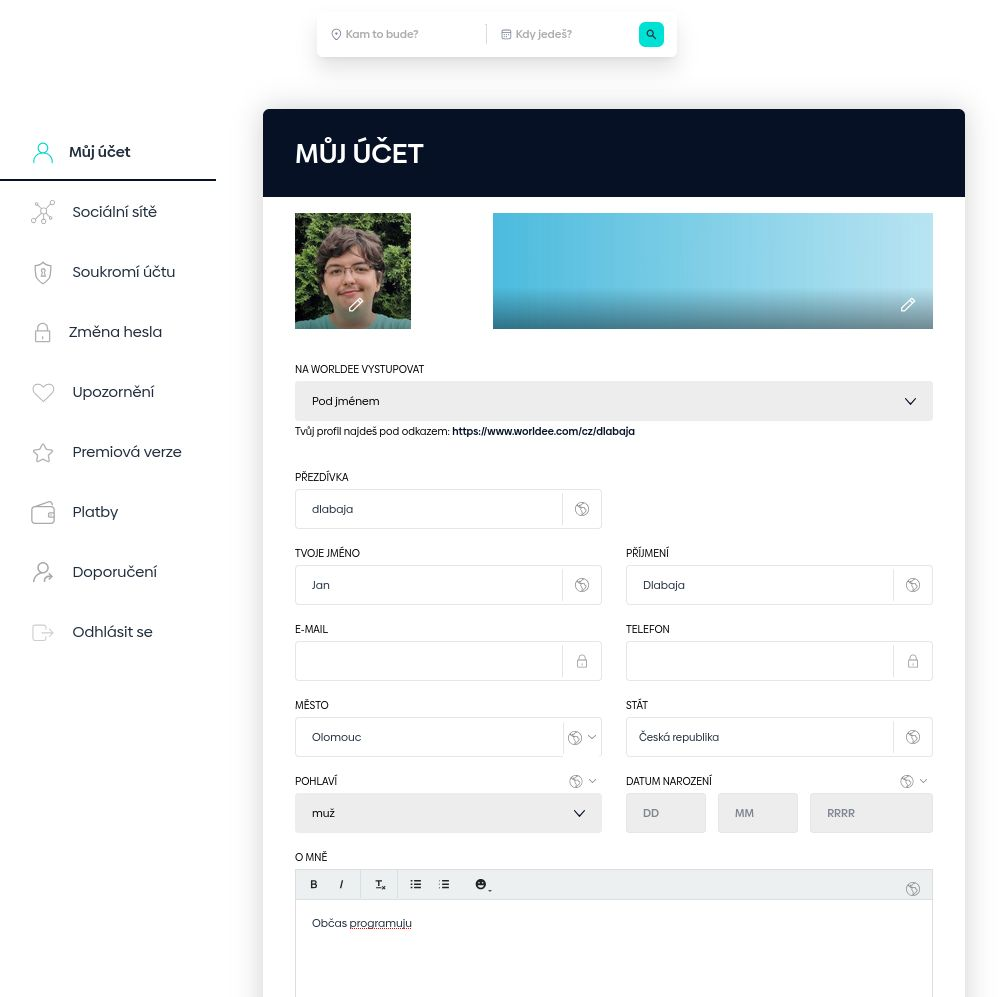
\includegraphics[width=0.7\linewidth]{obrazky/settings_old.png}
    \caption{Staré nastavení účtu napsané v Nette}
\end{figure}
\newpage
\section{Vizuální struktura stránky}

Celou stránku jsem rozdělil na levé menu a pravý kontejner, do kterého se bude vkládat obsah stránky.

\subsection{Komponenty}

Aby se dal projekt co nejlépe škálovat, shlukuje se kód do samostatných komponent. Takto se dá využívat na několika místech v projektu.

\subsubsection{Div}
Aby byly komponenty konzistentní, neměly by se nikdy stylovat zvenku. Můžete ale stylovat elementy, které je obalují. Díky obalení do \texttt{<div/>} tak najednou můžete komponenty posouvat, přidávat přes ně vrstvy, a různě s nimi manipulovat.

\subsubsection{FlexRow a FlexColumn}
Tyto dvě jednoduché komponenty jsem v rozvržení používal skoro všude. Mají na sobě flex box a dá se jim nastavovat řádkování, zarovnání obsahu, a kombinace sloupců a řádků umožňuje vytvořit jakkoliv komplexní design.

\subsubsection{Text}
Jedna z našich nejjednodušších komponent je obyčejný text. Dá se na něm měnit velikost, barva, tučnost, podtržení, a několik dalších vlastností. Pro nadpisy používáme Heading, který automaticky velikost textu přizpůsobuje rozlišení obrazovky.

\subsubsection{Ikona}
Na stránkách používáme dva typy ikon – Fluent ikony jsou externí (viz \href{https://fluenticons.co}{https://fluenticons.co}) a obsahují knihovnu několika tisíc piktogramů, které se dají použít téměř pro všechny účely. Ostatní ikony a obrázky, které knihovna nemá, si pak tvoříme sami, ve formátu SVG nebo PNG.

\subsubsection{Tlačítko}
Tlačítek můžete na webu najít osm druhů, každé z nich používá trochu jinou barevnou paletu (zelené, černé, transparentní, ...). Kromě textu podporují i ikony (zleva nebo zprava), velikost, dají se vypnout, a dokonce umí zobrazovat načítací animaci, kterou jsem použil pro odesílání dat formuláře.

Kromě toho máme vytvořené checkboxy nebo toggly, které na stránce s nastavením naleznete také.

\subsubsection{Link}
Do normálního odkazu musíte psát celou adresu. Do našeho se vkládá objekt ActionData, který ji reprezentuje a jeho předdefinované hodnoty zabraňují duplicitním a chybným url. Umí otevírat i soubory nebo stránky v novém panelu a je plně kompatibilní s Next.js - po najetí na něj pošle požadavek serveru na vykreslení další stránky, takže uživatel po kliknutí nemusí na nic čekat.

\subsubsection{Text box}
Základ této komponenty tvoří obyčejný \texttt{<input/>} element. Je ale obohacený o placeholder, který ze přesune nahoru, pokud má Text box nějaký obsah. Pokud je jeho obsah nesprávný, je možnost mu nastavit parametr errorMessage a tím ho celý nechat zčervenat, včetně malého textu s vysvětlením chyby pod boxem. Také se mu dá měnit typ (například na heslo), zda se do něj dá psát, nebo jeho velikost.

\subsubsection{Combo box}
Tato komponenta je užitečná pro výběr z předdefinovaných hodnot. Její základ tvoří knihovna react-select. Dá se v něm vyhledávat, má podporu i pro mobilní telefony a v projektu ho často používáme například pro výběr zemí, měn, nebo telefonních předvoleb.

\subsubsection{Text editor}
Někdy potřebujete text s formátováním. A rozdíl mezi normálním \texttt{<input/>} elementem a naší Text editor komponentou je srovnatelný s rozdílem mezi poznámkovým blokem a Wordem. A tím myslím i v komplexnosti, podobný editor jsem si zkoušel napsat sám a není to nic jednoduchého. Samozřejmá je podpora kurzívy, podtržení, i tučného písma, tvorba seznamů, hypertextových odkazů, i vestavěná klávesnice pro emotikony.

\subsubsection{Toast}
Toast je obdélníková komponenta, která se (většinou dole) zobrazí, aby uživatele informovala o vykonané akci. Například, zda se uložily změny, nebo naopak, že server neodpovídá.

\subsubsection{Swipeable drawer}
Díky této komponentě od mého oblíbeného Material UI můžeme poskytovat hezké rozhraní i pro mobil. Ačkoliv umí jen „vysunout“ obsah přes část stránky, používáme ji pro mobilní Combo boxy i Menu v nastavení a administraci. Aktivace probíhá kliknutím na tlačítko a zpět se zasune dotykem kamkoliv mimo sebe.

\subsubsection{Banner with editor}
První ze zmíněných komponent, kterou jsem částečně vytvořil sám. Původně šlo o banner na profilu, ale protože ho nikdo neplánoval znovu použít, veškerá logika pro úpravu fotky byla mimo něj. Vše se mi povedlo sjednotit a nyní se do něj jednoduše vkládají parametry jako fotka, akce při změně nebo smazání fotky, zda má tlačítko pro úpravy a také její výška, která se na obou stránkách liší.

\subsubsection{User icon with editor}
Ikona s uživatelskou fotkou měla ten samý problém co banner. Veškerá logika pro úpravu fotky byla součástí velké kompozice profilu. Pokud jste majitel profilu (nebo jen nastavíte parametr canEdit na true), můžete si jednoduše změnit vaši profilovou fotku.

\newpage
\subsection{Kompozice}

\subsubsection{Menu}
Inspirace pro menu vycházela z kompozice, která se už používala na stránce s Travel Buddy administrací. Protože ale nebyla uzpůsobená na to, aby se používala jinde, bylo na mě ji to „naučit“.

Mé nové menu bylo složené ze dvou části. První, horní, byla samotná navigace. Ta se od té původní zase tolik nelišila, jen jsem podle designu trochu upravil barvy. Jinak se jednalo o malou komponentu, do které šel vložit text, ikona, odkaz, akce po kliknutí, a zda je aktivní. Vše ovládala rodičovská komponenta AppMenu (pro desktop) nebo její potomek MenuRight (pro mobil), obě k tlačítkům ještě přidaly klíč, aby je React zvládnul lépe vykreslit. Druhá komponenta byl obrázek uživatele s jeho jménem a textem pro odhlášení. Přes ni byl daný odkaz, po jehož kliknutí byl uživatel odhlášen a vrácen na domovskou stránku.

Desktopovou verzi asi nemusím příliš popisovat. Horní část byla ve ScrollShadow komponentě, což poslední odkazy dokázalo skrýt, pokud by jich bylo hodně a nevešly by se na obrazovku. Zajímavější je ovšem verze pro mobil. Je totiž založená na již zmíněné SwipeableDrawer komponentě a dá se ovládat změnou proměnné open.

Pokud toto menu chcete kdekoliv použít, stačí mu předat menuItems parametr, složený z pole obsahujícího text na tlačítko, odkaz, ikonu a zda je aktivní (k tomu mi skvěle poslouží Next.js hook usePathname(), který vrací aktuální url). Změny, které se promění čistě na mobilu, zase předávám parametry isOpen, akci po zavření onClose a titulkem header.

\begin{figure}
    \centering
    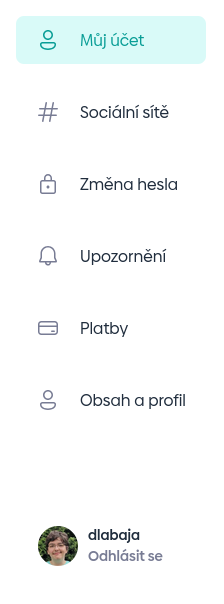
\includegraphics[width=0.5\linewidth]{obrazky/menu.png}
    \caption{Menu}
\end{figure}


\subsubsection{Account Container}
Protože má každá z podstránek stejnou horní část, a také, aby se mi lépe umisťovaly, vytvořil jsem pro každou z nich kontejner. Ten si podle aktuální cesty tvoří jméno stránky a v mobilní verzi se mu objevuje tlačítko, kterým se dá otevírat postranní menu. Do komponenty samotné se pak vkládají jednotlivé stránky, které Vám nyní představím.


\subsubsection{Podstránka Můj účet}
Stránka s účtem se dá označit jako srdce celého nastavení. Na první pohled Vás určitě zaujal banner přes celou stránku, o kterém již byla řeč. Jediný rozdíl oproti tomu na profilu je jeho výška, která je o 100 pixelů kratší. Hned pod ním se dá nastavit profilový obrázek.

Kromě toho jde na této stránce nastavit jméno, příjmení, přezdívku, pod čím chcete vystupovat, email, telefon, a sekci O mně, ve které se můžeme představit.

Ačkoliv komponenta s názvem města Olomouc vypadá jako jen další Text box, není tomu tak. Pokud do ní totiž začnete psát, začnou se vám díky Google Autocomplete funkci zobrazovat návrhy měst (případně i míst). Box vlastně ani neobsahuje text, ale objekt, jehož součástí jsou i GPS souřadnice daného místa.

Posledním boxem je již zmiňovaný Combo box se všemi státy světa.

Na konci celého nastavení leží tzv. Bookmark komponenta. Když ji rozbalíte, dostanete možnost odstranit Váš účet z Worldee.

Po kliknutí na tlačítko se otevře Modal – takové malé plovoucí okno. Tento konkrétní lze zavřít jen kliknutím na horní křížek nebo jedním ze dvou spodních tlačítek. Uvnitř jsou checkboxy, ve kterých uživatel vybere, proč chce Worldee opustit. Také může dolů do Text boxu napsat konkrétní důvod. Dole pak už jen potvrdí své heslo (pokud ho má) a kliknutím na tlačítko „Opustit Worldee“ bude odhlášen a přesměrován na hlavní stránku.

\begin{figure}
    \centering
    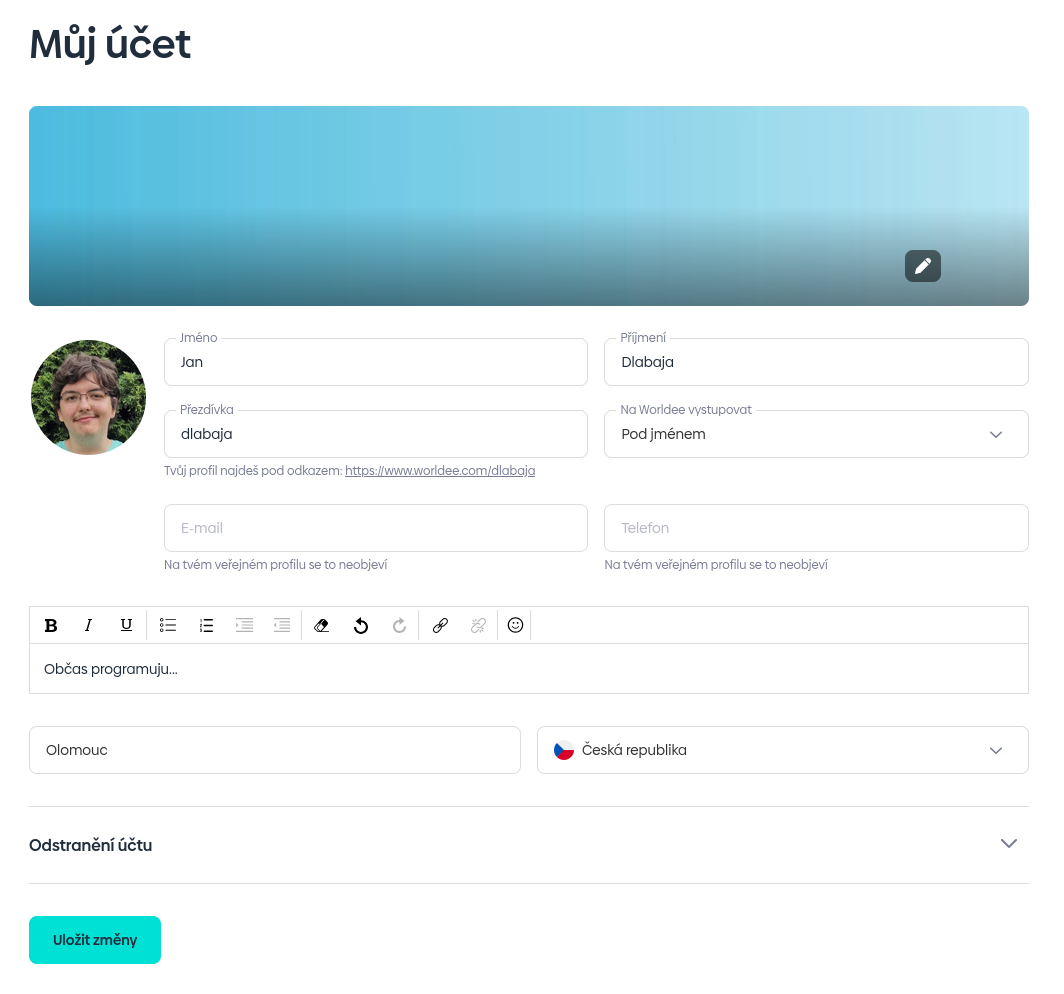
\includegraphics[width=1\linewidth]{obrazky/account.png}
    \caption{Podstránka Můj účet}
\end{figure}

\begin{figure}
    \centering
    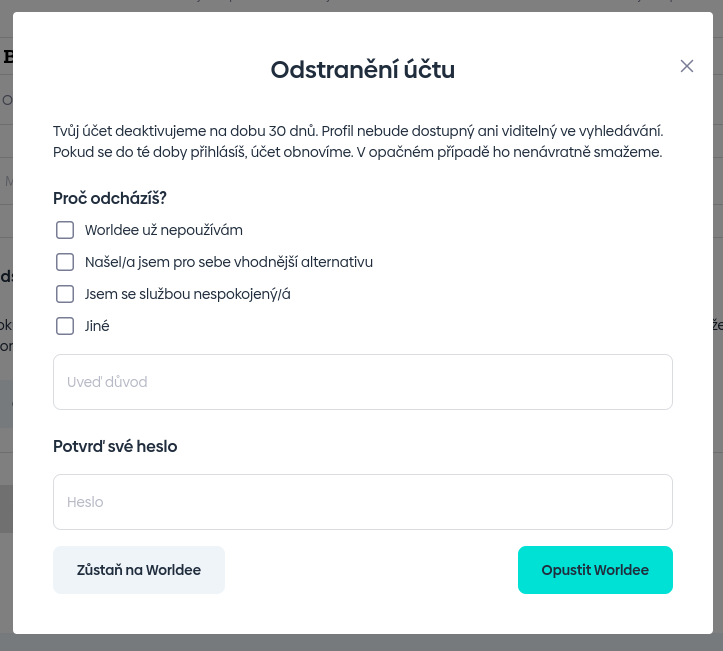
\includegraphics[width=1\linewidth]{obrazky/delete_account.png}
    \caption{Dialog s odstraněním účtu}
\end{figure}


\newpage
\subsubsection{Podstránka Sociální sítě}
Na této stránce si s Worldee můžete propojit svůj Facebook nebo Instagram účet, který se Vám pak objeví na profilu. Každá sociální síť se skládá z názvu, levé části a tlačítka. Pokud jste si ji zatím nepřipojili, bude levá část pouze Text box a pravá tlačítko „Propojit účet“. Pro propojení stačí napsat URL Vašeho profilu na jedné z těchto sítí. Pokud bylo úspěšné, Text box se změní na komponentu složenou z ikony a dvou textů oznamujících, že je účet propojen, a z původně zeleného tlačítko se stane tmavě šedé s názvem „Zrušit propojení“.

\begin{figure}[!h]
    \centering
    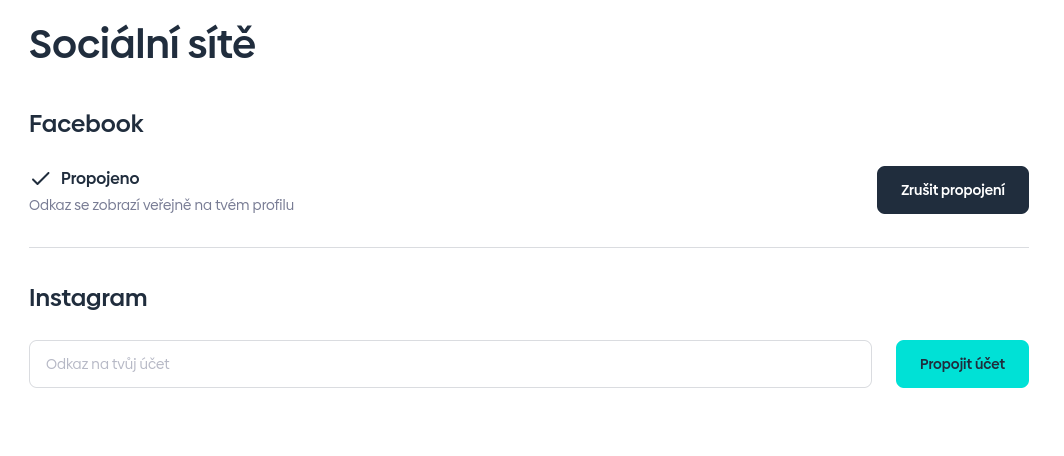
\includegraphics[width=1\linewidth]{obrazky/social_networks.png}
    \caption{Podstránka Sociální sítě}
\end{figure}


\newpage
\subsubsection{Podstránka Změna hesla}
Zatím jedna z těch jednodušších stránek – pouhá tři pole, jejichž typ je nastaven jako heslo, a text. Pokud jste přihlášeni přes přes službu třetí strany jako třeba Google, první pole se vám neukáže – ještě u nás totiž žádné heslo nemáte. Objeví se až po nastavení nového.

\begin{figure}[!h]
    \centering
    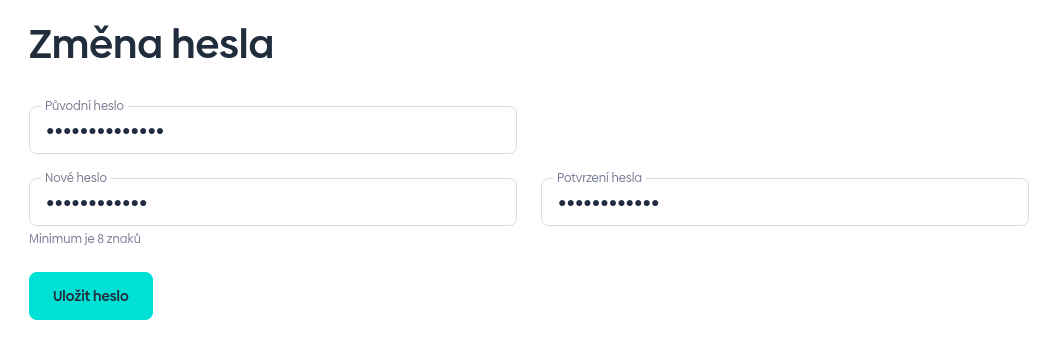
\includegraphics[width=1\linewidth]{obrazky/change_password.png}
    \caption{Podstránka Změna hesla}
\end{figure}


\newpage
\subsubsection{Podstránka Upozornění}
Tato kompozice se skládá ze dvou částí. Ta levá je velmi podobná té ze Sociálních sítí – jen má jiný obsah. Napravo je ale toggle tlačítko, kterým si uživatel může nastavit, z čeho chce (nebo nechce) dostávat webová upozornění.

\begin{figure}[!h]
    \centering
    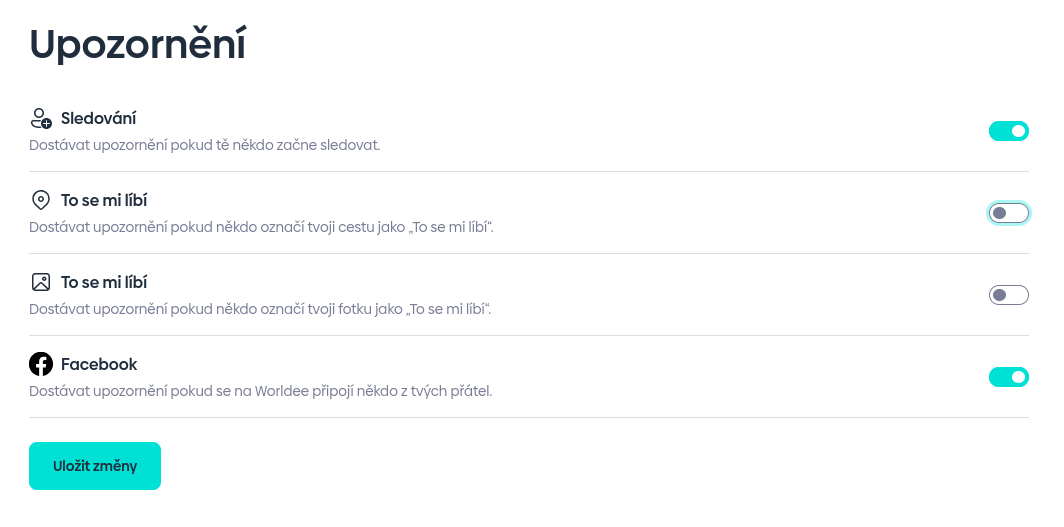
\includegraphics[width=1\linewidth]{obrazky/notify_settings.png}
    \caption{Podstránka Upozornění}
\end{figure}


\newpage
\subsubsection{Podstránka Obsah a profil}
A nyní poslední mnou vytvořená stránka. Je tvořená sekcí Profil a Zobrazení obsahu. V té první si můžete již známými Combo boxy vybrat, zda chcete, aby byl Váš profil viditelný pro všechny nebo jen pro vás. Hned vedle zase asijští zákazníci mohou přepnout střed mapy z Evropy na Asii.

Pod komponentami se nacházejí dva toggly. U horního si nastavíte, zda chcete schvalovat, když Vás někdo označí na jakékoliv fotografii, než se toto označení zobrazí na vašem profilu. Druhý toggle už se nachází v sekci Zobrazení obsahu a umožňuje Vám nejnovější cesty na Worldee zobrazovat ve feedu.

\begin{figure}[!h]
    \centering
    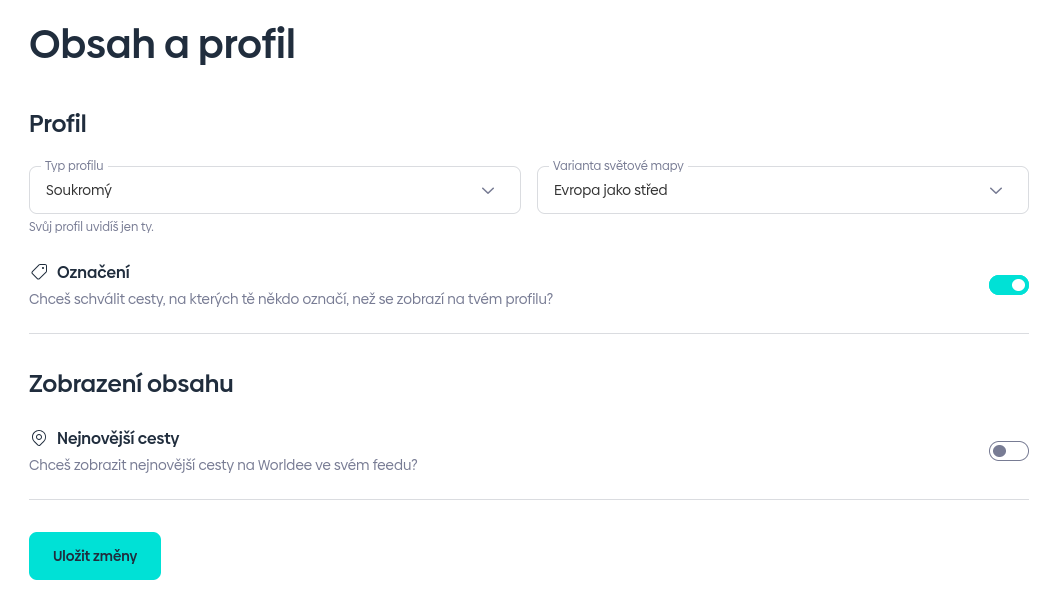
\includegraphics[width=1\linewidth]{obrazky/content_and_profile.png}
    \caption{Podstránka Obsah a profil}
\end{figure}


\newpage
\subsubsection{Podstránka Platby}
Poslední stránkou na seznamu je ta s platbami. Jako jedinou jsem ji nemusel psát úplně od základů, nicméně pár úprav bylo pro zakomponování do systému potřeba. Všechny className atributy jsem přesunul do <div /> elementů, načítání dat jsem připojil ke svému systému načítání stránky a proběhlo tak až po prvním renderu komponenty, a zmizela i přehnaně komplexní logika pro zobrazení plateb.
\\
\begin{figure}[!h]
    \centering
    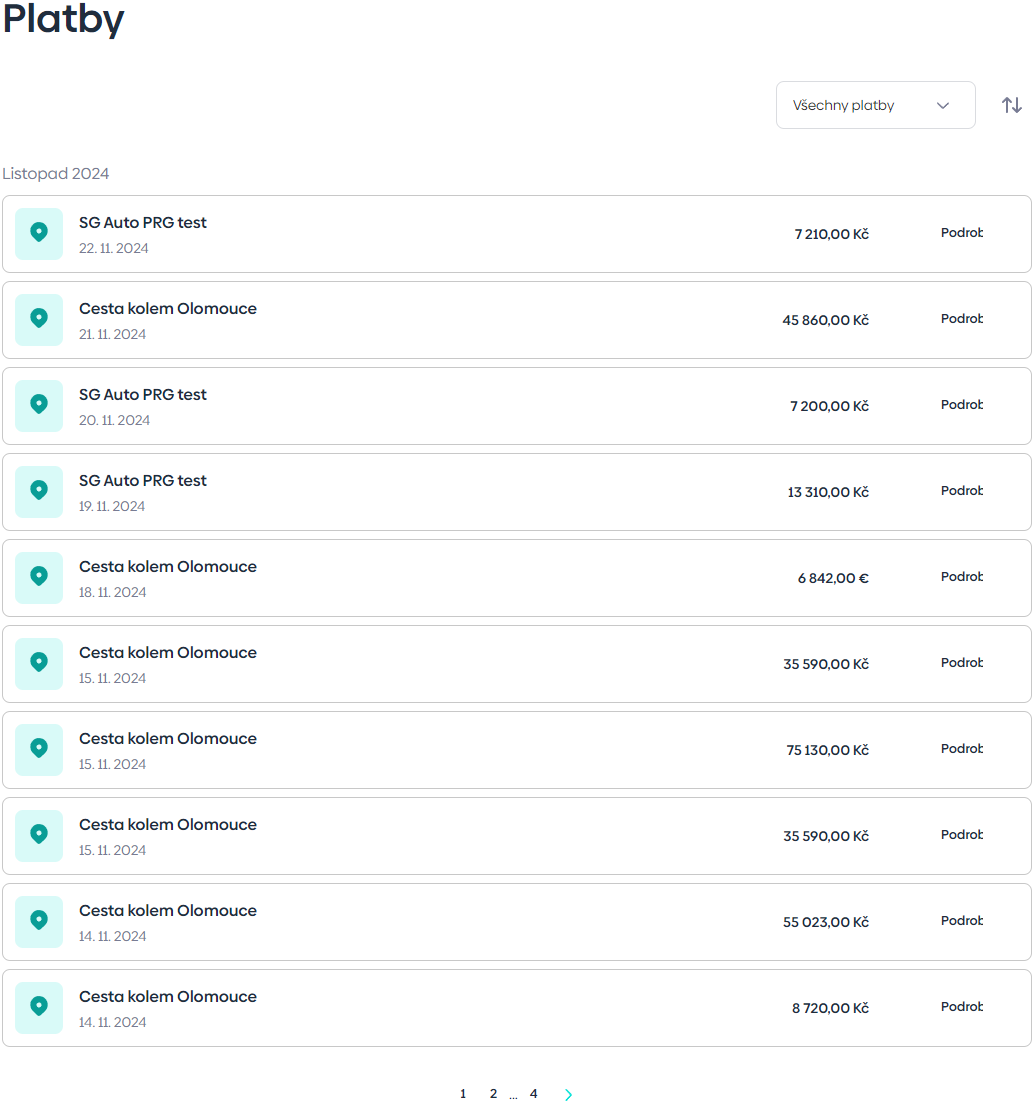
\includegraphics[width=0.9\linewidth]{obrazky/platby.png}
    \caption{Podstránka Platby}
    \label{fig:enter-label}
\end{figure}
\newpage
\newpage
\section{Datová struktura stránky}

Kdyby byl celý web tvořen jen vizuálními prvky, moc by toho nedělal. O vizuálním stavu stránky se špatně píše, protože většinou stačí pro dosažení cílového vzhledu jen naskládat několik komponent na sebe. To zajímavé, co sice normální uživatel nevidí, ale bez čeho by stránka nefungovala, je její datová část. Díky ní můžete reprezentovat, jaká mají prvky data, jak jsou propojené, a jak spolu celá architektura funguje.

\subsection{MobX store a validace dat}
Jak funguje MobX už víte. Asi vás proto nepřekvapí, že svůj vlastní store má každá z již vyjmenovaných stránek. Díky tomu nemusím používat useState() a kazit si tak svá data Reactem.

Store stránek je třída složená z polí obsahujících všechna data, která se budou na stránce používat, jejich náležitých getterů (a většinou i setterů) a konstruktoru. Všechna pole, která se mění, musí být označena dekorátorem @observable a jejich změna musí být obalená buďto v runInAction() funkci nebo @action dekorátoru.

Konstruktor by měl správně jen dosadit základní hodnoty, spustit nějaké interní funkce a zavolat makeObservable(this), čímž aktivuje MobX. Externí data z API by ho mohly zbrzdit nebo vyvolat vyjímku, proto by si je měl vývojář zavolat sám. Proto má každá ze stránek svoji veřejně přístupnou metodu init(), která se v Reactu volá po prvním renderu. Tím ovšem vzniká další problém – když se stránka načte, ještě nemá data. Proto jsem si vytvořil vlastní funkci load(), kterou všechny stránky používají, spolu s isInitialized stavem. Ten se změní, jakmile se všechna data načtou, a díky tomu vím, kdy stránku zobrazit uživateli, a kdy ji nahradit načítací animací.

Každý ze storů má dvě speciální pole. FormChanged se nastaví na true po tom, co změníte jakákoliv data na stránce – třeba vlastní přezdívku. Tím se Vám zároveň odemkne tlačítko s odesláním dat, čímž jsem alespoň částečně zabránil tomu, aby náš server zaplňovaly prázdné požadavky. Jakmile data odešlete, formChanged se opět nastaví na false a tlačítko zamkne.

FormLoading se zase nastaví na true po tom, co data uložíte. Zamkne všechna pole, aby hodnoty zůstaly během odesílání konzistentní, a zůstane tak, dokud server nepošle odpověď.

Pokud je na stránkách potřeba nějaké volání na API, i to naleznete zde. Kromě metody init() a save(), které jsou všude, mají některé stránky i své vlastní metody – třeba na smazání a nahrání fotky v nastavení účtu, nebo připojení Facebooku a Instagramu v sociálních sítích.

U nastavení účtu a změny hesla jsem se nevyhnul ani validaci dat. Pokaždé, když kliknete na tlačítko pro uložení, spustí se metoda validate(). Ta aktualizuje hodnoty jako nicknameIsValid, nebo emailIsValid podle toho, zda nejsou prázdné nebo v neplatném formátu. Getterem isValid() se dá následně zjistit, zda validace prošla.

Pokud bylo vráceno true, spustí se část, kterou mají všechny stránky stejnou – funkce save(). Podobně jako load() bere jako argument metodu, kterou má spustit (každý store má kromě init() i svůj save()), a také již zmíněné formLoading a formChanged, se kterými podle odpovědi serveru manipuluje. Ať už je odpověď jakákoliv, vždy se dole zobrazí Toast, díky němuž uživatel zjistí, zda se operace zdařila, server neodpovídá, nebo se například neshodují hesla.
\newpage
\subsection{Data, konvertory a API}
Postupně se dostávám výš a výš v naší frontendové hierarchii. Všechna data, která jsem dostával ve storu, jsou vlastně jen datové třídy. Konkrétně se jedná o třídy s definovanými poli reprezentujícími jejich obsah, gettery, a konstruktorem, jehož jediný parametr je interface se všemi dosaditelnými hodnotami, kterým třídu můžeme naplnit. Protože nemá settery, jde to jen jednorázově, a tak veškeré změny proměnných řeší až store a já zde nemusím používat MobX a @observable dekorátory.

Zhruba na stejné úrovni jako data mohou být i konvertory. Ne vždy jsou totiž data z databáze v pro nás ideálním formátu. Například čas i enumy jsou vyjádřené jako string, s čímž se ale špatně pracuje a museli bychom ho před každým použitím převést. Stejné je to i s různými objekty. Konverze probíhá ještě před tím, než se vše vloží do datové třídy, takže na stránce dostávám takovou strukturu dat, se kterou už můžu jednoduše pracovat. Přenos zpátky probíhá podobným způsobem, jen je třeba data zase převést na serverem podporovaný formát.

Ještě výš se nachází námi zpracované metody pro práci s API. Jsou systematicky rozdělené do několika tříd podle místa použití, abych, pokud potřebuji pracovat s nastavením, nemusel importovat něco, co má navíc funkce pro získání nejnovějších cest, přihlášení uživatele, a vrácení posledních hodnocení na Googlu. Každá metoda přijímá kromě dat také parametr na úpravu požadavku, díky kterému můžu měnit jeho hlavičku, cookie, nebo zda chci, aby při chybě stránka nespadla, a já si tak mohl vyjímku odchytit sám.

Každá z metod nakonec zavolá funkci importovanou z api.ts souboru. Tento soubor o délce přes čtyřicet tisíc řádků se automaticky generuje pomocí nástroje Swagger, a skrývá reálnou API implementaci, která je vlastně jen soubor všech možných HTTP požadavků, které fungují jako most mezi frontendem a backendem. Výš už pro mě cesta nevede.

Ve Storybooku je struktura trochu odlišná. API funkce se volají stále stejně, ale při načtení jakékoliv story se jejich původní implementace přepíší na mock. Ten vrací mock datové třídy, díky čemuž nejsou potřeba žádné konvertory. Abychom alespoň částečně simulovali internetovou odezvu, každá z metod vrací data až po uplynutí doby 300 milisekund.
\newpage
\subsection{Unit testy}
Abychom si byli jistí, že web funguje správně alespoň po datové stránce, máme pomocí Jestu (a dříve Karmy) napsaných několik stovek testů. Všechny jsou ve složce test, která má úplně stejnou strukturu jako složka s komponentami, jen s tím rozdílem, že všechny soubory mají příponu .spec.ts.

Každá datová část se testuje trochu jinak. Aktuálně nejvýše v hierarchii jsou testy na datové třídy. Protože jsou neměnné a dají se naplnit jen jednou, je potřeba jen vyzkoušet, zda se data dosadila správně. To jde zjistit pomocí tvorby falešných dat, jejich dosazením a následně porovnáním všech veřejných getterů.

Testům se samozřejmě nevyhnou ani konvertory. Zde konkrétně byl potřeba jen jeden, a to pro první stránku s uživatelským nastavením. Testy jsou z principu podobné těm datovým, opět jen stačí vytvořit falešná data, ty dát do konvertoru, a pak zkontrolovat data nového objektu, který od něj dostaneme.

Poslední a největší skupina testů se zaměřuje na samotné komponenty a jejich MobX store. Zároveň jsou také nejkomplexnější, protože musí pokrýt všechno od přidávání a získávání dat, validací a komunikací s API.

Stejně jako u ostatních typů se i tady kontroluje dosazení do konstruktoru a následný stav. Kromě toho se ale proměnné zkouší nastavit již mimo konstruktor a zkoumají, zda správně funguje setter. Na všech stránkách se ve většině setterů nastavoval i formChanged parametr, který byl také potřeba do testů zahrnout.

Validace už je docela komplikovaná. Například u přezdívky se jen stačilo ujistit, že není prázdná. Email už zase musel mít správnou strukturu. A AppearAs, Combo box, který určoval, zda budete viditelní pod přezdívkou nebo pod jménem, si musel být jistý, že při výběru „Pod jménem“ byla správně nastavená alespoň jednu část jména a „Pod přezdívkou“ zase požadoval nastavenou přezdívku, která se validovala v předchozím kroku.

Následně se testují všechny metody integrující API volání. Ačkoliv jsou všechny z nich jen mocky a ve skutečnosti na server nevolají, můžu vyzkoušet, zda se pod nimi zabalená API metoda zavolala s těmi parametry, které jsem jejímu rodiči předal. K tomu se výborně hodí SpyObject.
\newpage
\subsection{Architektura webu}
Pro lepší představu o funkci webu vám nyní vysvětlím, co všechno se stane, pokud stránku navštívíte.

Vše začne zadáním adresy \href{https://www.worldee.com}{worldee.com} do adresního řádku (1). Požadavek se odešle na náš Next.js server, kde si ho jako první převezme middleware. Ten zkontroluje a případně upraví cookies a hlavičky požadavku a do url přidá lokalizaci. Potom ho předá routeru, který podle url najde většinou již předkreslenou požadovanou stránku, přeloží ji a posílá zpátky do prohlížeče (2).

Pokud byla stránka předem předkreslená, uživatel už nyní může vidět všechny její prvky, ač jde zatím jen o vizuál postrádají jakoukoliv funkčnost. Pokud ne, stránka je prázdná. Prohlížeč musí spustit React (3), stránku inicializovat a podle odpovědi serveru vytvořit všechny kompozice a komponenty. Po prvním renderu začíná probíhat komunikace s naším PHP serverem (4) a získaná data jsou z JSONu převáděna na použitelný formát (5), kterým jsou plněny datové třídy. Stránka je nyní plně načtená, celý proces trval jednotky sekund. 

\begin{figure}[!h]
    \centering
    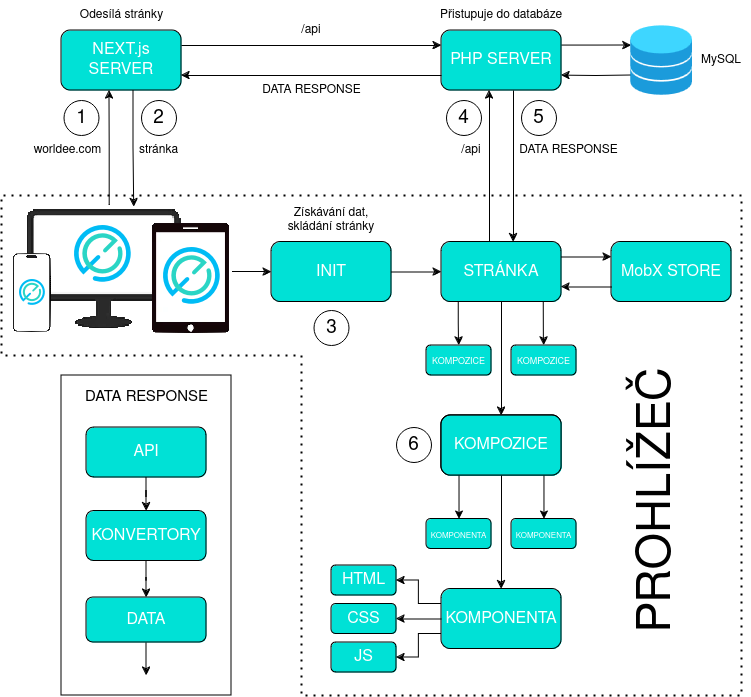
\includegraphics[width=1\linewidth]{obrazky/architektura.png}
    \caption{Diagram architektury webu. Zdroj: vlastní práce.}
\end{figure}
\clearpage


\newpage
\newpage
\section{Finální vzhled stránky}

\begin{figure}[h!]
    \centering
    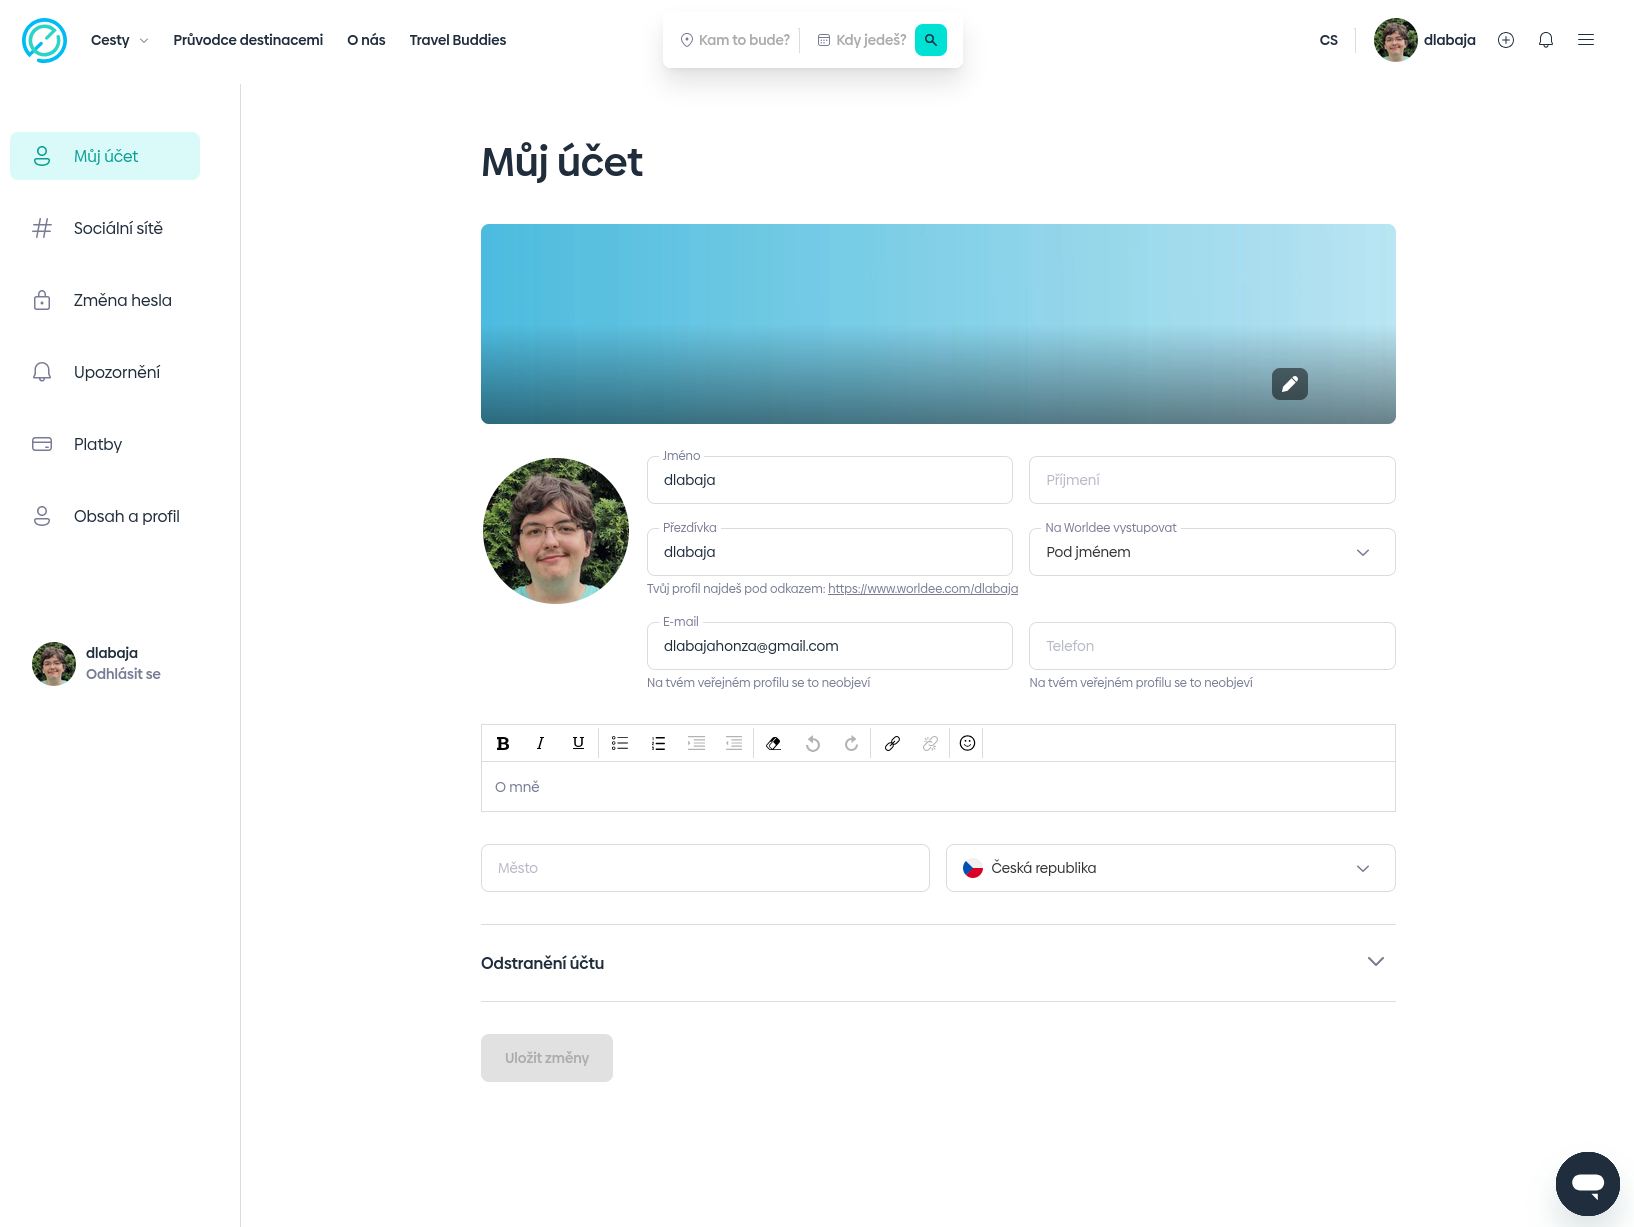
\includegraphics[width=1\linewidth]{obrazky/finalni_stranka.png}
    \caption[Vizuální podoba stránky]{Vizuální podoba stránky, dostupná po přihlášení na \\\href{https://www.worldee.com/cz/settings/account}{www.worldee.com/settings/account}}
\end{figure}
\newpage

    \chapter{Články v časopisu Elektronka}
Ačkoliv se nejedná o podmínku hodnocení této práce, pro lepší pochopení této problematiky jsem začal psát články pro \href{https://www.spseol.cz/prace-zaku-a-studentu/casopis-elektronka}{školní časopis Elektronka}\cite{Elektronka} a obohacoval jimi tak svou rubriku \href{https://github.com/dlabaja/IT_doupe}{IT doupě}\cite{ITDoupe}. První vznikl v záři 2024 a mým úkolem je popsat od základů vytvořit web s tím, že každý měsíc do něj implementuju jinou technologii. Od primitivní HTML stránky se tak postupně dostávám k bundlingu, Reactu, Next.js, nebo lokalizacím.

\begin{figure}[!h]
    \centering
    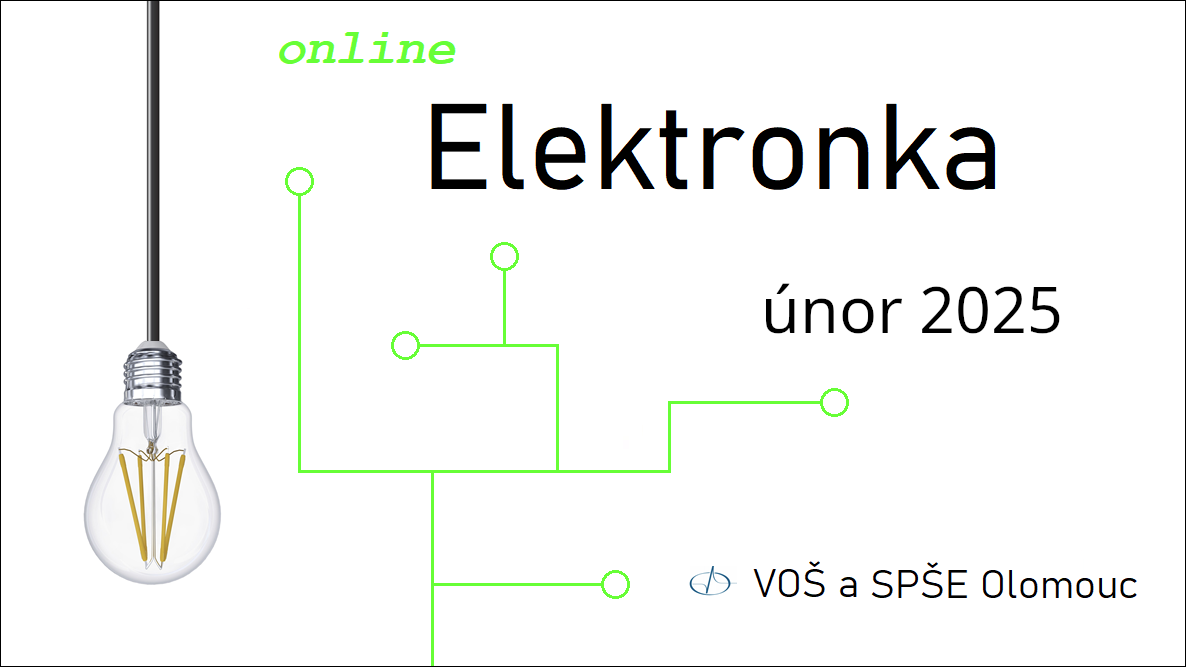
\includegraphics[width=1\linewidth]{obrazky/elektronka.png}
    \caption{Titulní obrázek časopisu Elektronka (únor 2025).\cite{Elektronka}}
\end{figure}

     % Pokud je nutné přidat kapitolu, vytvořte soubor .tex ve složce kap a poté zde zadejte příkaz \include{cesta k souboru}. Název zvolte jaký chcete, ale v žádném případě v názvech nepoužívejte mezery ani diakritiku!
    \chapter*{Závěr}\addcontentsline{toc}{chapter}{Závěr}\markboth{Závěr}{}

Jak jste asi zjistili, svět webu je komplikovanější, než se může na první (nebo i druhý) pohled zdát. Už dávno mezi sebou neposíláme statické HTML dokumenty a s příchodem stylů, JavaScriptu, JQuery, a prvních frontendových frameworků se toho hodně změnilo. Nové, někdy opravdu revoluční knihovny vycházejí téměř na denní bází a je stále těžší držet krok. Dokonce i popsané technologie jsou jen špička ledovce a je dost možné, že za pár let už některé z nich ani nebudou existovat.

A ačkoliv jsou nové technologie komplikované, díky jejich abstrakci je psaní a hlavně následné škálování webu mnohem jednodušší než dřív. Místo šablon používáme komponenty a kompozice, místo stylů CSS moduly a Tailwind, JavaScript je typově bezpečný, zkompilovaný kód je díky bundlerům malý a efektivní, před chybami nás chrání testy, lokalizaci můžou překladatelé dělat přes webové rozhraní, a spoustu dalších větších a menších vylepšení pro uživatele i vývojáře.

Po dopsání tohoto projektu jsem se účastním vývoje i jiných částí webu. Opravil a vyčistil jsem Text editor, vytvořil komponentu s telefonním číslem a výběrem předvolby, přidal vyhledávání do mobilního Combo boxu, nebo mapuju data ze scraperu na naše API. Tvorba webů je něco, v čem jsem se momentálně našel, a co ještě nějakou chvíli budu dělat. A chtěl bych poděkovat celému vývojovému týmu, že mi pomáhají na cestě za jeho pochopením.
    %------------------------------------------------------------------------------------------------------------------------------ 
    % % Neměňte tuto část
         
    %--- Citace
\fancypagestyle{plain}{
					\fancyhf{}								
					\fancyfoot[R]{\helv \thepage}			
					\renewcommand{\headrulewidth}{0.4pt}
					\renewcommand{\footrulewidth}{0.4pt}
				}

\newpage
\clear

\renewcommand{\bibname}{Seznam použitých zdrojů}
\addcontentsline{toc}{chapter}{Seznam použitých zdrojů}
\printbibliography


%--- Seznam obrázků
\newpage
\clear
\addcontentsline{toc}{chapter}{Seznam obrázků}
\listoffigures


%--- Seznam tabulek
\newpage
\clear
\addcontentsline{toc}{chapter}{Seznam tabulek}
\listoftables

 %, seznam obrázků a tabulek - neměnit
    \appendix

\chapter*{Přílohy}\addcontentsline{toc}{chapter}{Přílohy}
\renewcommand{\thesection}{\arabic{section}} % arabské číslice

\section{Plakát}
\begin{figure}[!h]
    \centering
    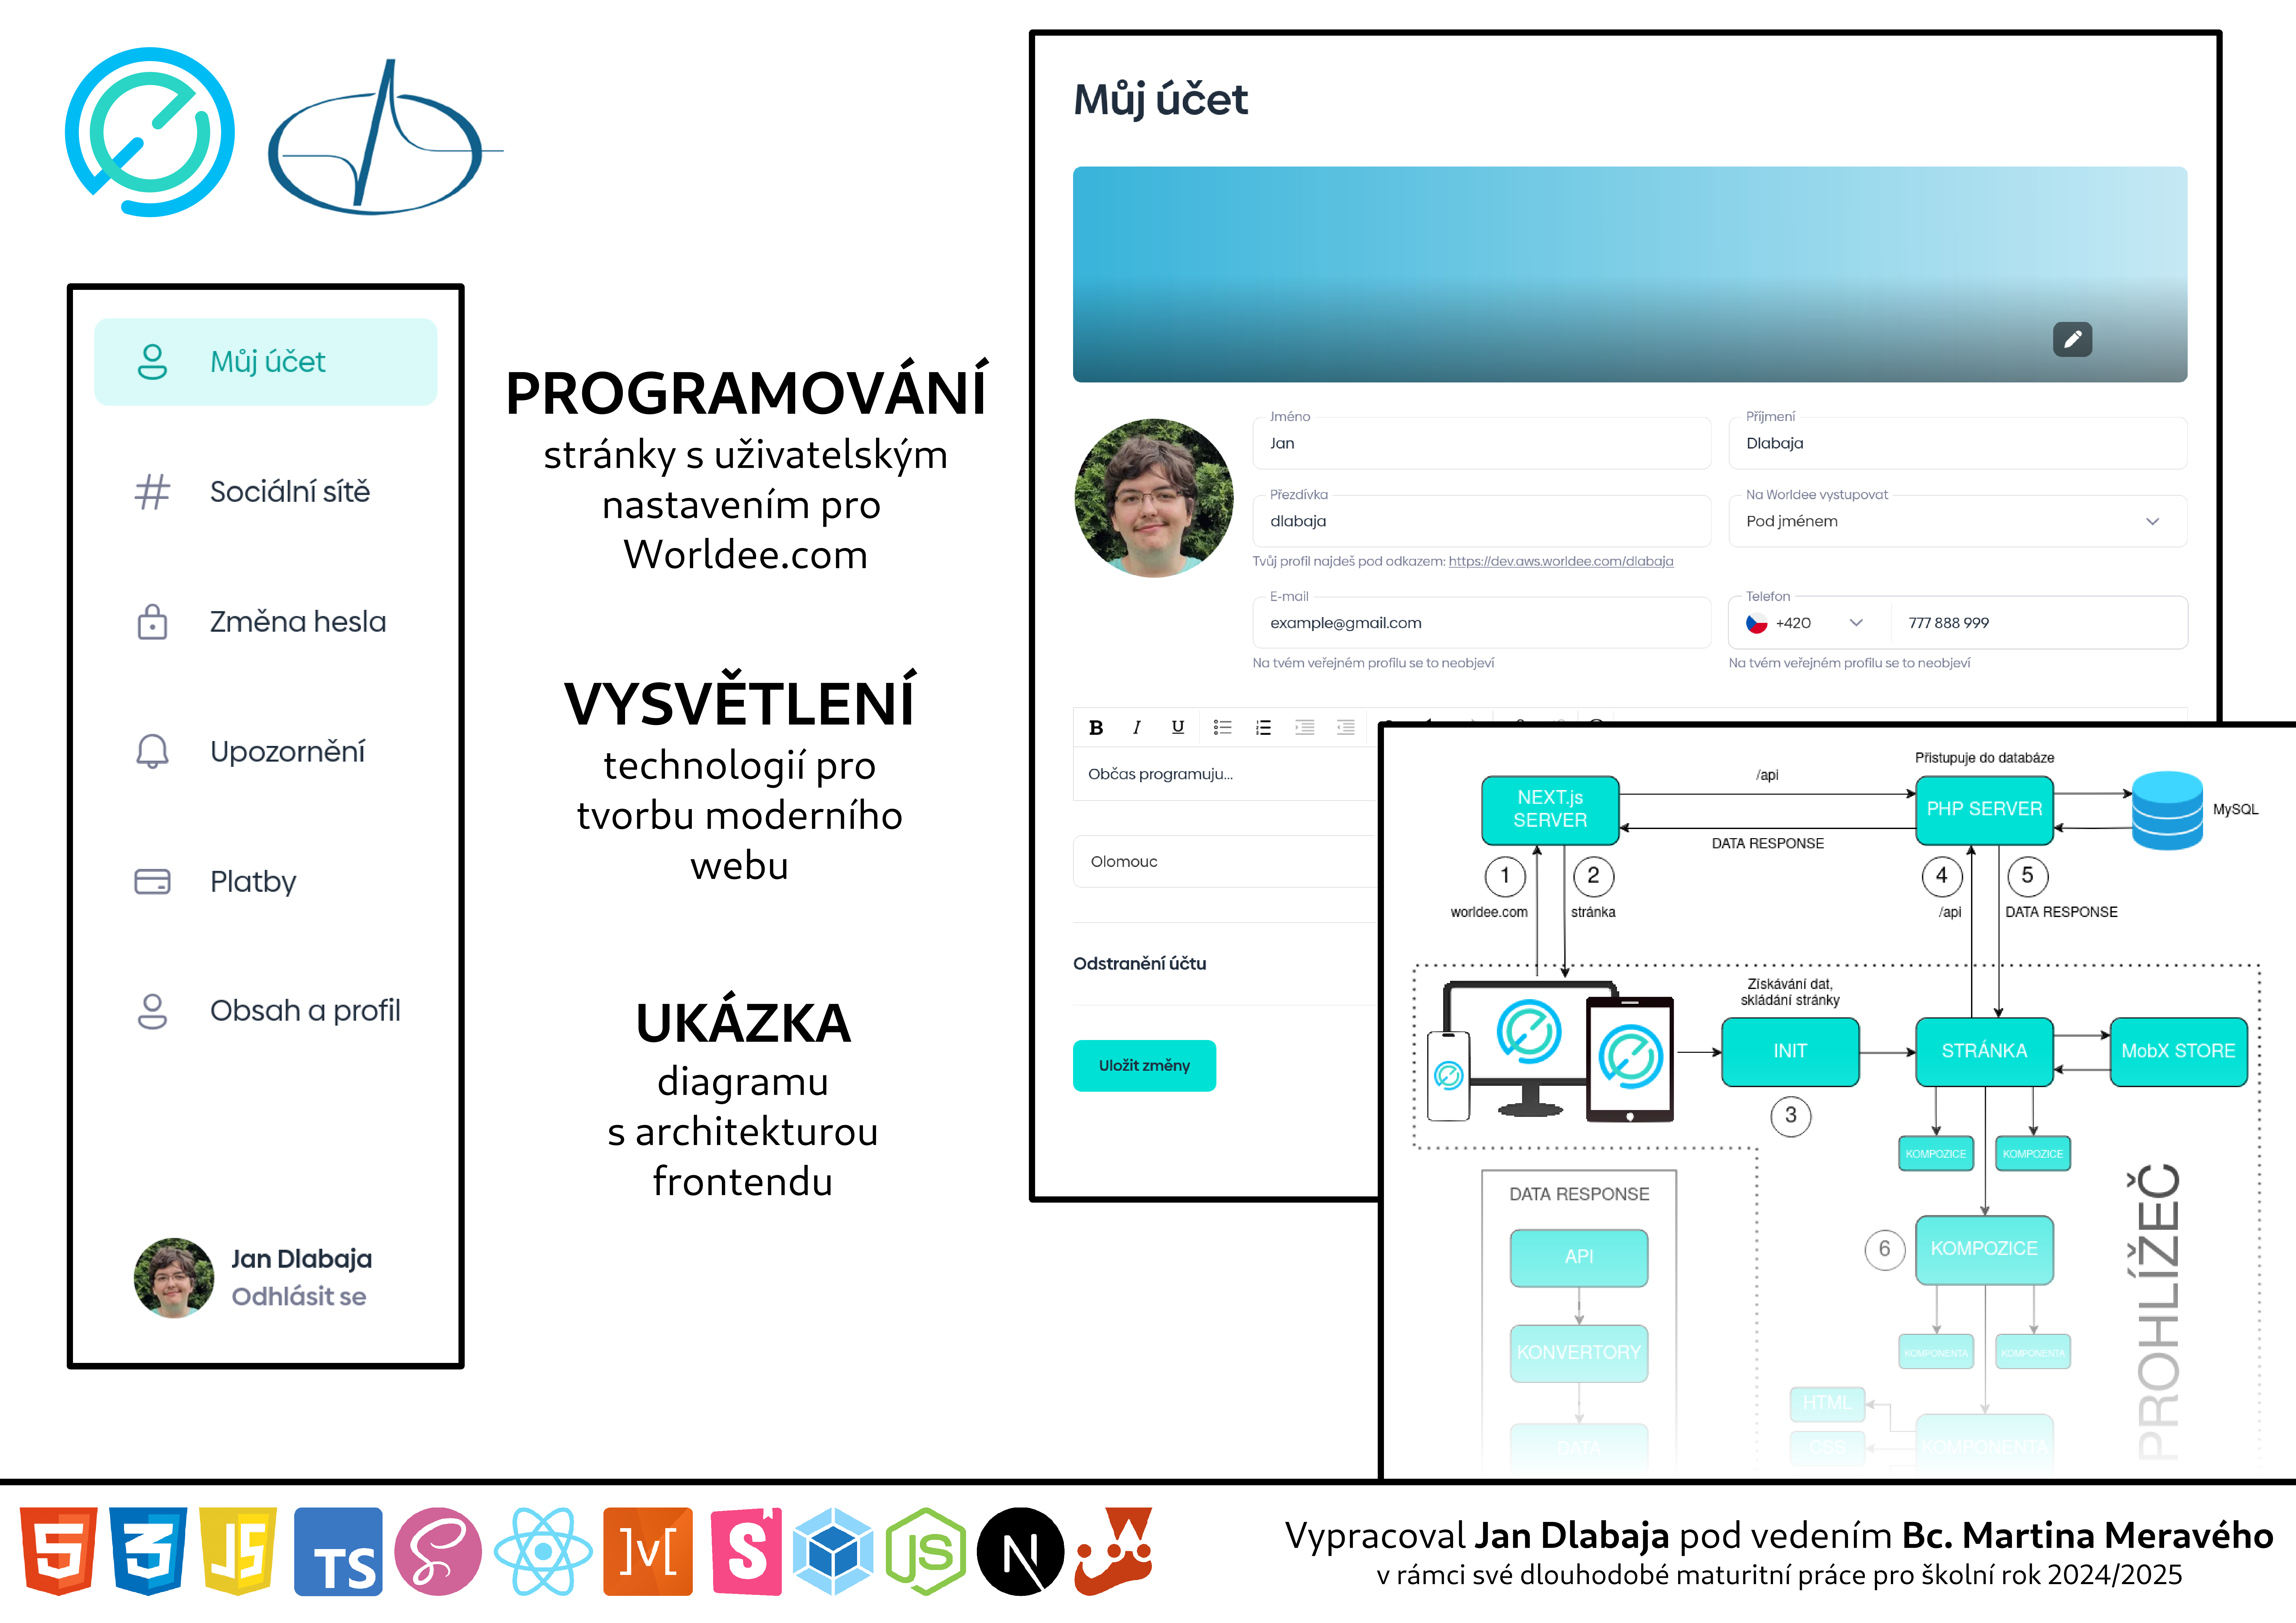
\includegraphics[width=1.2\linewidth, angle=90]{obrazky/plakat.png}
    \label{fig:plakat}
\end{figure}
\end{document}
